\documentclass[review,3p,times]{elsarticle}
\usepackage[utf8]{inputenc}
\usepackage[T1]{fontenc}
\usepackage{amsmath,amssymb}
\usepackage{graphicx}
\usepackage{booktabs}
\usepackage{tabularx}
\usepackage{array}
\usepackage{threeparttable}
\usepackage{adjustbox}
\usepackage{lineno}
\usepackage{setspace}
\usepackage{placeins}
\usepackage{caption}
\usepackage{url}
\usepackage[hidelinks]{hyperref}
\graphicspath{{../figures/}}
\captionsetup{font=small,labelfont=bf,labelsep=period,justification=raggedright,singlelinecheck=false}
\renewcommand{\arraystretch}{1.15}
\emergencystretch=2em
% float placement: keep tables and figures close to their first citation
\renewcommand{\topfraction}{0.9}
\renewcommand{\bottomfraction}{0.7}
\renewcommand{\textfraction}{0.08}
\renewcommand{\floatpagefraction}{0.75}
\setcounter{topnumber}{3}
\setcounter{bottomnumber}{2}
\setcounter{totalnumber}{4}
% float pages: start at the top margin instead of centring the floats
\makeatletter
\setlength{\@fptop}{0pt}
\setlength{\@fpsep}{16pt plus 2pt}
\setlength{\@fpbot}{0pt plus 1fil}
\makeatother
\journal{Tourism Management Perspectives}
\def\refitem#1{\noindent\hangindent=1.5em\hangafter=1 #1\par\medskip}
\begin{document}


\begin{frontmatter}
\title{Revenue without residual claims: Contract design and the revenue--profit
divergence in China's listed tourism firms}
\author[a]{Yuan Zhao\corref{cor1}}
\ead{zhaoyuan@hist.edu.cn}
\author[b]{Yingtao Ji}
\ead{jiyingtao@hist.edu.cn}
\author[b]{Mengjie Hu}
\ead{hmj@hist.edu.cn}
\author[c]{Songmei Liu}
\ead{liusongmei@xxgc.edu.cn}
\author[b]{Chenyu Yang}
\ead{yangcy@hist.edu.cn}
\affiliation[a]{organization={School of Foreign Languages, Henan Institute of Science and Technology},
  city={Xinxiang}, postcode={453003}, country={China}}
\affiliation[b]{organization={School of Music and Dance, Henan Institute of Science and Technology},
  city={Xinxiang}, postcode={453003}, country={China}}
\affiliation[c]{organization={School of Humanities and Law, Xinxiang Institute of Engineering},
  city={Xinxiang}, postcode={453003}, country={China}}
\cortext[cor1]{Corresponding author.}
\begin{abstract}


Listed tourism firms can report rising revenue while net profit falls. This paper asks where that gap forms and whether disclosed contracts help explain it. Using 24 A-share listed tourism firms over 2015--2025 (264 firm-years), 16.7\% of observations with calculable growth paired rising revenue with falling net profit (15.9\% among the 17 continuously disclosing firms); measured on growth rates the shares are 28.3\% and 26.5\%. A five-component decomposition of 225 firm-years locates the gap below the operating layer. For 13 firms observed in both subperiods, the operating-layer margin rose from 30.60\% to 38.29\%, while the parent-attributable net margin fell from 11.19\% to \ensuremath{-}4.77\%; minority interest, interest, impairment and depreciation together added 23.65 percentage points of deductions. We then hand-collect 99 contract clauses from 32 reports issued by seven firms. The notes table contains no scenic-area contract, whereas five scenic-area clauses appear only in the main text; one set of five Qujiang clauses equals 20.72\% of half-year consolidated revenue. Panel estimates for 115 firm-years with continuous disclosure associate interest and impairment negatively, and depreciation positively, with net margins; the positive depreciation coefficient may reflect a common-denominator effect. We read these patterns as consistent with \emph{revenue without residual claims}: a contractual allocation in which the operator appears to recognise revenue while holding a limited claim on incremental receipts and continuing responsibility for asset-related costs. The evidence remains associative, and the contract sample is small, so the interpretation may be treated as provisional.

\end{abstract}
\begin{keyword}
value capture \sep revenue rights \sep cost obligations \sep tourism firms \sep contract disclosure \sep China
\end{keyword}
\end{frontmatter}
\linenumbers


\section{Introduction}

Revenue and profit do not move closely together in the financial statements of China's listed tourism firms. Across the sample of 24 A-share listed tourism firms over 2015--2025, comprising 264 firm-years, 16.7\% of observations with calculable growth pair rising revenue with falling net profit (40/240). The pattern is also present among the 17 firms classified as A-level, that is, firms with continuous disclosure and comparable statement items. These firms contribute 187 firm-years, including 170 with calculable growth, of which 15.9\% exhibit this divergence (27/170). Measured on growth rates the shares are 28.3\% and 26.5\%; the difference arises from firm-years whose prior-year profit was negative, where a percentage change reverses sign (Section 4.1). The correlation between revenue growth and net-profit growth is only 0.129, compared with a level correlation of 0.552. These descriptive relationships do not establish why profits fail to follow revenue, but they motivate a distinction between recording revenue and retaining its economic benefits. We argue that the divergence is not only a demand or operating-efficiency problem. It is also potentially a value-capture problem rooted in the contractual allocation of revenue entitlements and cost responsibilities. In particular, an operator may recognise revenue without holding a substantial claim on the additional receipts generated by expanding activity, while remaining responsible for the assets and financing that support it.

Demand fluctuations, cost rigidity and pandemic disruption provide plausible explanations for weak profitability. Tourism expenditure does not translate mechanically into income retained by any particular enterprise, a distinction consistent with the broader separation between tourism spending and its economic effects (Dwyer et al., 2004). The pandemic also disrupted tourism activity and business organisation, making period comparisons especially sensitive to changing conditions (Sigala, 2020). These explanations remain relevant, but they do not fully account for the accounting pattern examined here. Among 13 A-level firms represented in both subperiods, the operating margin rises from 30.60\% in 2015--2019, based on 46 observations, to 38.29\% in 2020--2024, based on 51 observations. Over the same comparison, the net margin attributable to the parent, defined as net profit attributable to parent divided by operating revenue, falls from 11.19\% to \ensuremath{-}4.77\%. The four deductions examined---minority interest, interest, impairment, and depreciation and amortisation---expand by 23.65 percentage points in total: 2.98, 2.06, 7.00 and 11.61 points, respectively. The divergence directs attention beyond operating performance towards the conversion of operating returns into earnings attributable to the parent. It does not demonstrate improved technical efficiency, nor imply that every deduction lies below operating profit in statutory presentation. It does suggest that operating weakness alone is an incomplete account.

The theoretical distinction between value creation and value capture provides a starting point for interpreting this gap (Bowman \& Ambrosini, 2000; Lepak et al., 2007). Creating value does not ensure that the organisation undertaking an activity appropriates the resulting returns; complementary assets, bargaining positions and industry arrangements shape their distribution (Coff, 1999; Jacobides et al., 2006; Teece, 1986). We apply this distinction through two contractual concepts. A revenue right is the contractual entitlement to a revenue stream, such as ticket revenue, a management fee or a sharing payment. A cost obligation is the contractual and legal responsibility for the asset base and its financing, depreciation, maintenance and impairment. A residual claim is an entitlement to the revenue remaining after prior contractual entitlements have been satisfied, including the relevant share of incremental receipts. Revenue recognition does not, by itself, establish such a claim. We define asymmetric appropriation as a contractual allocation in which the party recognising revenue lacks a claim on the surplus that revenue generates while bearing the cost obligation of the asset base. Property-rights theory helps frame the separation of asset responsibilities, contractual entitlements and residual control (Grossman \& Hart, 1986; Hart, 1995). Our emphasis is narrower: revenue-sharing arrangements must be assessed alongside the costs that remain with the operator. The cost side can be obscured when value capture is inferred from reported sales or contractual payment shares without examining asset-related obligations.

Chinese scenic-area concessions and entrusted-management arrangements provide a setting in which this distinction is consequential. A local government or scenic-area authority may retain the underlying revenue right while remunerating the listed operator through a cost-based management fee. Alternatively, a stepwise sharing schedule may reduce the operator's marginal share at higher revenue levels. Where the operator also carries the asset base, depreciation, interest and impairment exposure, additional tourism activity need not yield a commensurate increase in retained earnings. We describe this configuration as ``revenue without residual claims''. The phrase identifies a contractual mechanism, not a claim that all operators lack residual entitlements. Research on public--private partnerships likewise stresses that payment structures and risk allocation are interdependent design choices (Engel et al., 2014; Iossa \& Martimort, 2015). Tourism governance research directs attention to the public institutions that organise economic participation (Hall, 2011). To examine these arrangements, we hand-collected 99 contract clauses from 32 reports issued by seven firms. Disclosure occurred through two channels: 94 clauses appeared in the notes table and five in the main text. The notes table contained no scenic-area contracts; the five scenic-area clauses appeared only in the main text. In the 2024 half-year, one set of five Qujiang clauses totalled RMB 159.6228 million, equivalent to 20.72\% of half-year consolidated operating revenue. This example illustrates potential financial materiality and the limitations of relying on a single disclosure channel.

Three questions organise the study. The first (RQ1) concerns how often revenue growth fails to reach profit growth. The second (RQ2) concerns which accounting deductions sit between operating performance and parent-attributable earnings. The third (RQ3) concerns whether disclosed contractual arrangements are consistent with an asymmetric allocation of revenue rights and cost obligations. We address these questions through three measurement layers. The nominal-share layer examines reported amounts and contractual entitlements relative to revenue, distinguishing the scale of recognised activity from the share potentially retained. The period-change layer compares margins and deductions across subperiods to locate the widening gap in the financial statements. The marginal-association layer examines how cost burdens are associated with net margins across firms and years, without treating that association as an estimate of contractual effects. Together, these layers connect financial outcomes with disclosed contractual provisions while preserving the distinction between an accounting pattern and an explanatory mechanism. The contract sample is small and hand-collected, and disclosure availability limits its coverage. We do not claim causal identification, sector-wide contractual representativeness or that asymmetric appropriation explains every instance of falling profit. Instead, we assess whether the observed financial patterns and contractual evidence support a value-capture interpretation alongside demand, financing, ownership and operational explanations.

The paper makes four related contributions. Theoretically, it extends the application of value-capture reasoning in tourism by treating revenue rights and cost obligations as a joint allocation rather than equating recognised revenue with appropriated value. This formulation makes explicit how contractual limits on revenue participation can coexist with continuing asset-related exposure. Methodologically, the three-layer approach separates nominal shares, period changes and marginal associations, reducing the risk of interpreting revenue scale as evidence of successful value capture. The use of both notes-table and main-text disclosures also shows why contractual analysis requires attention to where information appears, not merely whether a report contains it. Empirically, the study documents the revenue--profit divergence in China's listed tourism firms and relates it cautiously to a bounded set of contractual observations. Practically, it suggests that investors, operators and public principals should assess payment schedules together with financing, depreciation, maintenance and impairment responsibilities. Higher visitor receipts or reported revenue alone are insufficient grounds for judging the financial sustainability of an operating arrangement. The remainder of the paper develops the conceptual framework, describes the sample and measurement procedures, presents the financial and contractual evidence, and discusses its implications and limitations for tourism governance and firm-level value capture.

\section{Theoretical background and propositions}

\subsection{Value capture and the revenue-side bias}

Value creation and value capture concern different economic relationships. Value creation refers to the benefits generated through an activity, whereas value capture concerns the portion appropriated by a particular participant (Bowman \& Ambrosini, 2000; Lepak et al., 2007). A tourism destination may create value for visitors, businesses and public authorities without generating commensurate returns for its operating company. Increased visitation or revenue does not, by itself, demonstrate improved capture. For listed tourism firms, the relevant question is how activity translates into earnings attributable to shareholders after contractual claims and associated obligations have been accommodated.

The appropriation literature explains why participants retain different portions of jointly created value. Control over complementary assets can strengthen a firm's position when commercialising an offering (Teece, 1986), while stakeholder bargaining can redirect returns away from shareholders even where the firm possesses valuable resources (Coff, 1999). Industry architecture also shapes bargaining positions by organising interdependencies and the distribution of activities across firms (Jacobides et al., 2006). These perspectives imply that revenue generation and shareholder appropriation need not coincide. Appropriation is also a governance problem: what shareholders retain depends on the claims that other participants hold and on the mechanisms that enforce them (Jensen \& Meckling, 1976; Shleifer \& Vishny, 1997). The operator delivering a tourism experience may remain dependent on a resource owner, infrastructure provider or public authority whose claims constrain its retained return.

Nevertheless, accounts of capture often foreground a participant's revenue share, contractual payment or bargaining outcome, giving cost allocation less analytical attention. This is a relative emphasis, not an absence of costs from the literature. Its limitation becomes apparent in asset-heavy, contract-bound tourism operations, where access to receipts may be accompanied by maintenance, financing and investment commitments. Two operators receiving the same revenue share can retain very different earnings if one must renew infrastructure and service project debt while the other receives an unencumbered management fee. A revenue-side measure can misidentify the economic beneficiary of increased activity.

Property-rights and transaction-cost approaches provide a basis for bringing these obligations into the analysis. Ownership and residual control influence investment incentives, contractual adaptation and exposure to costs that cannot be fully specified in advance (Grossman \& Hart, 1986; Hart, 1995; Williamson, 1985). Ownership alone does not determine every liability, but its interaction with contract terms helps establish who must respond when assets deteriorate or operating conditions change. We accordingly treat value capture as the outcome of jointly allocated revenue rights and cost obligations, rather than as a revenue entitlement considered in isolation.

\subsection{Revenue rights, cost obligations and asymmetric appropriation}

A \emph{revenue right} is an enforceable entitlement to a specified receipt or share of receipts generated by an activity. A \emph{cost obligation} is a contractual or ownership-linked responsibility to fund, incur or absorb specified expenditure and losses associated with that activity. A \emph{residual claim} is an entitlement to the economic surplus remaining after prior claims and obligations have been satisfied. \emph{Asymmetric appropriation} arises when the allocation of revenue rights and cost obligations gives a participant unequal exposure to the activity's upside and downside. The asymmetry of interest here combines restricted participation in incremental receipts with relatively open-ended responsibility for costs. Because contracts cannot specify every future contingency, the allocation of residual control and the parties' relational understanding carry much of the governance burden (Baker et al., 2002; Williamson, 1979).

Recognising revenue is not equivalent to holding a residual claim. An operator may recognise a contractual management fee or revenue from services it controls while retaining only a limited portion of additional destination receipts. Its accounting revenue may increase because reimbursable expenditure increases, rather than because its economic entitlement improves. Conversely, a resource owner may participate in incremental receipts without recognising the operator's sales. Revenue is thus an accounting measure of transactions within a reporting entity; residual participation depends on the enforceable distribution of surplus. The distinction becomes particularly important when destination receipts, project-company revenue and consolidated revenue refer to different economic boundaries.

Crossing the breadth of revenue rights with the scope of cost obligations yields four archetypes. In an aligned high/high arrangement, broad participation in incremental receipts accompanies extensive responsibility for operating and investment costs. In an aligned low/low arrangement, a narrow fee entitlement accompanies limited obligations. Neither alignment guarantees profitability, but the operator's upside and downside are broadly matched. A revenue-rich/cost-light arrangement provides substantial participation in receipts while placing major obligations elsewhere. The opposite, revenue-poor/cost-heavy arrangement, is the focal case: the operator recognises revenue but bears the cost obligations of the asset base without a corresponding claim on the surplus that revenue generates. The phrase in our title, \emph{revenue without residual claims}, is shorthand for this configuration; it does not assert that shareholders hold no residual claim at all. These are analytical categories rather than mutually exclusive legal forms. Figure 1 summarises the mapping and distinguishes the contract boundary, at which revenue rights are assigned, from the reporting boundary, at which costs and claims enter the consolidated statements.

\begin{figure}[!htbp]
\centering
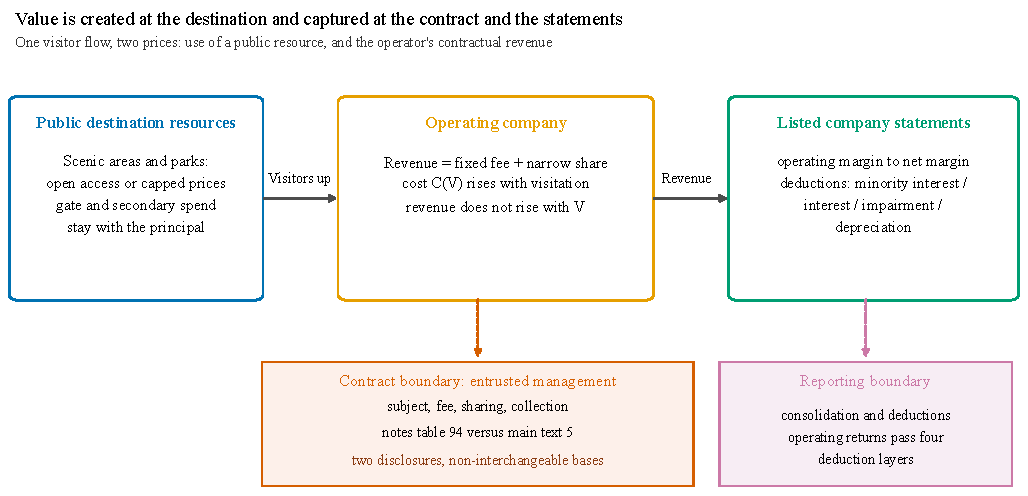
\includegraphics[width=0.95\textwidth]{../figures/en_fig1_mechanism.pdf}
\caption{Value creation at the destination and value capture at the contract and reporting boundaries. Visitor flows enter the operating company; revenue is assigned under entrusted-management agreements; operating returns pass through four deduction layers before reaching shareholders. Dashed lines mark the contract boundary and the reporting boundary.}\label{fig:1}
\end{figure}

The focal arrangement constitutes a potential value-capture failure, not simply a high-cost business model. High expenditure can be compatible with successful capture where additional activity generates a sufficient retained surplus. Under asymmetric appropriation, however, contractual restrictions can limit that surplus while leaving the operator exposed to financing needs, asset renewal or unrecovered expenditure. Demand determines the volume of activity, but the contractual allocation conditions the mapping from activity to retained earnings. Strong demand may therefore coexist with weak shareholder returns. This interpretation does not establish contractual inefficiency: an arrangement may support conservation or public access while limiting capture by the listed operator.

Incomplete-contract theory helps explain why such exposure cannot be inferred from a stated revenue percentage alone. Contracts cannot anticipate every investment requirement or contingency, making residual control and adaptation consequential (Hart \& Moore, 1990; Hart, 1995). In public--private arrangements, incentives depend on how operating responsibilities, investment decisions and risks are bundled and allocated (Engel et al., 2014; Hart, 2003; Iossa \& Martimort, 2015). Cost-based payment can protect against specified expenditure while weakening participation in demand-related gains; fixed payments can instead leave significant cost risk with the operator. The implications depend on reimbursement coverage, adjustment mechanisms and enforceability, not merely the contract's label.

Accounting introduces a further distinction between the reporting boundary and the contract boundary. Consolidation can bring a project's revenue, liabilities and expenses into group accounts even where some returns belong to non-controlling shareholders. IFRS 15 and CAS 14 address revenue recognition, including principal-versus-agent considerations, but recognised revenue does not independently establish residual entitlement (International Accounting Standards Board [IASB], 2014; Ministry of Finance of China, 2017). IFRIC 12 addresses qualifying service concession arrangements, while IFRS 16 addresses leases; their application can affect the presentation and timing of asset-related charges (IASB, 2006, 2016). Applicability depends on the arrangement's substance. These standards neither dictate contract terms nor mechanically identify capture failure, but they explain why similar-looking revenue totals can represent different economic positions.

\subsection{The Chinese scenic-area contract setting}

Chinese scenic-area operations provide a setting in which public resource control and corporate operating responsibilities can be separated. For the public scenic resources considered here, local governments or scenic-area authorities act as principals, while operating companies undertake specified commercial and managerial activities. Ticket-price regulation, conservation requirements and public-service commitments qualify the operator's commercial discretion. Chinese tourism policy has been shaped by state actors whose objectives extend beyond the commercial returns of individual operators (Airey \& Chong, 2010), and the resulting arrangements place distributional questions inside public institutions. State direction can extend to the construction of the destination itself, with land, capital and operating rights organised through local state vehicles (Ong \& Liu, 2022), and integration policies have been assessed for their effect on tourism development rather than on the returns of listed operators (Jin et al., 2022). This institutional structure is consistent with tourism governance perspectives that locate participation and distribution within public institutions, rather than treating destinations as collections of autonomous firms (Bianchi, 2018; Bramwell \& Lane, 2011; Hall, 2011). Its significance lies in the possibility that responsibility for delivering services exceeds control over their monetisation.

Concession and entrusted-management arrangements can combine fixed fees, cost-based remuneration, stepwise sharing, minimum guarantees and revenue sharing with maintenance or investment obligations. These provisions must be interpreted jointly. A minimum guarantee may protect an operator's income or protect a principal's receipts, depending on who provides it. A cost-based fee may reimburse eligible expenditure without covering financing costs or unapproved investment. A stepwise schedule may allow receipts to increase while reducing the operator's marginal share. The revenue base to which such a fee applies is itself regulated and spatially differentiated rather than set by the operator (Wang et al., 2021), and conservation requirements can impose measurable cost obligations on the operator of a scenic resource (Yang et al., 2020). Maintenance and investment clauses can also extend exposure beyond the current reporting period. Consequently, contract classification alone is insufficient: the relevant unit of analysis is the combination of payment, expenditure and adjustment provisions. Fee-oriented, asset-light arrangements have been examined as a source of value in lodging, where shifting asset ownership away from the operator supports capital structure and returns (Li \& Singal, 2019; Sohn et al., 2013). Asset ownership and fee entitlement have since been measured as separate dimensions of lodging groups (Lussi et al., 2023; Märklin \& Bianchi, 2022), and the fee schedule itself is treated as a strategic pricing decision rather than a by-product of the contract form (Sun \& Lee, 2024). The contracts studied here display the fee side of that arrangement without its asset-light counterpart: the fee is retained while the assets and their financing stay with the operator.

Listed operators are often state-owned enterprises or local state-controlled vehicles, with scenic-area activities conducted through consolidated project subsidiaries. Ownership in such firms is typically concentrated, and control rights can exceed cash-flow rights, so claims held by parties other than the listed shareholder are economically large (Claessens et al., 2000; La Porta et al., 1999). Local governments may simultaneously influence resource access, corporate governance and contractual remuneration. Policy implementation in Chinese tourism is mediated by local discretion and by coordination across agencies (Wang \& Ap, 2013), which bears on how remuneration terms are set and how they are enforced. Research on fiscal decentralisation and official incentives provides grounds for examining how local revenue needs and development objectives enter these relationships, without assuming a uniform effect across locations (Jin et al., 2005; Li \& Zhou, 2005; Qian \& Weingast, 1997). Evidence concerning political connections and related-party arrangements similarly motivates attention to governance and intragroup claims; it does not establish that scenic-area contracts necessarily transfer value away from listed shareholders (Fan et al., 2007; Jiang et al., 2010). Common public ownership does not by itself eliminate distributional differences between the authority, the listed company and other claimants. Firm-level work on Chinese listed tourism companies relates performance to governance and technical efficiency (Peng et al., 2021), and meta-analytic evidence summarises the antecedents of hospitality and tourism firm performance more broadly (Lim \& Ok, 2021); in both strands revenue and profit enter as interchangeable outcomes, so a gap between them is not the object of explanation. Contractual partnerships and corporate restructuring have been examined for their financial consequences (Dewally \& Gordon, 2022; Li et al., 2022), and the performance of tourism firms also responds to attributes of the asset base that contract terms do not record, such as the environmental quality of the site (Cheong et al., 2024).

Contract visibility is also institutionally structured. Two relevant disclosure channels are the standardised notes table for entrusted management/contracting and the narrative ``other material contracts'' section. The table offers a consistent classification but may omit scenic-area arrangements reported under another contractual category. The narrative section is less standardised yet can disclose economically important remuneration, sharing, guarantee or investment clauses. This is a possible feature of the reporting architecture, not a claim about every firm or reporting period. Disclosure research supports distinguishing the availability of information from its comparability and interpretability (Healy \& Palepu, 2001; Schipper, 2007), and the reporting of revenue-related measures has been shown to affect how users process firm performance (Blankespoor et al., 2022). In the Chinese setting, mandatory operating-information disclosure has been found to change related-party transaction behaviour (He et al., 2025), which indicates that disclosure rules shape what these contracts look like in the record. An empty table cannot therefore establish that the firm lacks material scenic-area obligations; assessment requires reading both channels.

\subsection{Propositions}

\emph{P1 (prevalence).} We expect revenue growth and growth in profit attributable to the parent to diverge in a substantial minority of firm-years. Restricted incremental revenue rights and continuing cost obligations provide the mechanism: expanding activity need not produce proportionate shareholder earnings. This expectation applies where contractual asymmetry is economically material; it is not a numerical prevalence claim derived from theory. Broadly matched revenue and profit movements would be inconsistent with the proposition.

\emph{P2 (location).} We expect the divergence to sit in the deduction layer, not in the operating margin. That layer comprises non-controlling interests, interest, impairment, depreciation and amortisation. This expectation is conditional on operating performance remaining comparatively stable while financing, asset and ownership claims absorb returns. The layer is an analytical bridge, not a statutory subtotal: depreciation and impairment may enter operating profit, while non-controlling interests allocate profit rather than constitute expenses. Comparisons must therefore avoid double counting. Divergence explained predominantly by deterioration in a consistently constructed operating margin before the identified charges would be inconsistent with the proposition.

\emph{P3 (contract design).} We expect cost-based fees and stepwise shares with declining marginal rates to coincide with low fee-to-revenue ratios and with cases in which recognised fees remain unsettled. Here, the ratio compares the operator's fee entitlement with the underlying scenic-area revenue to which the fee relates. The mechanism requires fees to rise more slowly than activity and collection to depend on approval, reimbursement or settlement. Cost-based remuneration alone does not imply payment delay. Proportional or increasing fee participation combined with prompt settlement would be inconsistent with this expectation.

\emph{P4 (cost obligation).} We expect interest and impairment burdens to be negatively associated with net margins. Depreciation intensity may carry a positive coefficient where asset-base differences and denominator effects dominate. Interest and impairment absorb current earnings; higher depreciation intensity may also identify asset-rich operations with stronger earnings capacity, while shared revenue denominators can influence observed associations. This possibility does not imply that depreciation improves profitability. The expectation is conditional on comparable accounting definitions and asset composition. A robust negative depreciation association after accounting for these features, or no negative interest and impairment associations, would be inconsistent with the proposed pattern.

\emph{P5 (disclosure).} We expect economically material scenic-area contracts to be more likely to appear in narrative disclosure than in the standardised entrusted-management/contracting notes table. The mechanism is classification mismatch: material arrangements may warrant narrative explanation without being entered under the table's narrower reporting category. This expectation applies where both channels are available and contracts are assessed for economic materiality independently of disclosure location. Equally comprehensive or more complete coverage in the notes table, or consistent duplication across both channels, would be inconsistent with the proposition.

P1 corresponds to RQ1, P2 to RQ2, and P3 to P5 to RQ3. The propositions are examined through three complementary measurement layers: nominal share, period change and marginal association. Nominal shares describe how reported revenue is distributed across earnings and identified claims at a given time. Period changes assess whether revenue expansion coincides with improved retained earnings. Marginal associations examine how variation in contractual or accounting burdens relates to capture measures, subject to accounting identities, denominator effects and observational limitations. These layers are not substitutes: a low nominal share does not establish deterioration, growth divergence does not identify its contractual source, and an association does not demonstrate causality. Their joint interpretation provides a more disciplined assessment of the value-capture gap.

\section{Data and measurement}

\subsection{Sample and evidence map}

The financial panel comprises 24 A-share listed tourism firms observed over 2015--2025, representing 264 firm-years (Appendix Table A1). Revenue and profit growth are calculable for 240 firm-years. The primary sources are public annual and semi-annual reports filed by the listed firms. Financial items and contract disclosures were hand-collected and cross-checked against the reported financial statements. Because 2025 is a partial-disclosure year, its observations are not treated as a complete annual reporting cohort. Their inclusion in the descriptive panel does not establish comparability with full-year observations.

Firms are classified according to disclosure completeness and statement comparability, not financial performance. The A-level group contains 17 firms with continuous disclosure and comparable statement items, comprising 187 firm-years, of which 170 have calculable growth. The B-level group contains 4 firms and 44 firm-years; the C-level group contains 3 firms and 33 firm-years. Both groups remain in the full-sample description but are not merged into the A-level statistics. This separation preserves the distinction between coverage of listed tourism firms and the narrower evidence supported by comparable accounting items.

Accounting data for the decomposition cover 2015--2024 and contain 225 firm-years. All five components are available for 165 observations. The remaining 60 have at least one missing component recorded as zero and flagged; Appendix Table A6 classifies those missing items by origin and reports the sensitivity of the estimates to zero substitution. The main decomposition uses the complete cases. Zero substitution in the flagged records is a computational convention, not evidence that the relevant firm incurred no interest, impairment, or depreciation and amortisation burden. These observations must remain distinguishable from records containing reported zeros.

A-level observations form the regression frame: 170 firm-years over 2015--2024 (17 firms \ensuremath{\times} 10 years). Of these, 115 enter the estimation. Fourteen firm-years lack a usable revenue denominator in the financial-statement panel: 13 are absent from the panel (eight from 2015, when annual-report coverage is incomplete, and five belonging to firms listed after 2015), and one (002627 in 2017) reports no revenue. Of the 156 firm-years with a revenue denominator, 41 lack at least one regressor: 24 lack interest expense, 20 lack both impairment items, and three lack both interest expense and impairment items. The 115 observations are therefore a listwise-deletion sample rather than a complete A-level panel. Growth comparisons use a different window. A within-firm growth rate requires two adjacent years, so the 2015 observations cannot supply one and the growth frame runs from 2016 to 2025: 170 A-level firm-years (17 firms \ensuremath{\times} 10 years) and 240 in the full panel. The growth frame and the regression frame therefore coincide in size but not in coverage. Three frames are in use --- 156 firm-years with a revenue denominator (the parent of the regression sample), 165 complete decomposition cases, and 170 growth observations --- and each is defined by a different availability requirement; none is a successive screening stage of another.

Divergence is classified by the signs of the two level changes, revenue and parent-attributable net profit, between adjacent years of the same firm. A percentage growth rate is reported alongside as a descriptive companion, but it is not used for classification: a rate computed on a negative prior-year value reverses sign, so a narrowing loss would enter as falling profit and a widening loss as rising profit. Section 4.1 reports both criteria and the number of cases affected.

Three analytical questions organise the evidence map. Table 1 describes the coverage and revenue--profit growth patterns of the 24-firm panel, with 264 firm-years and 240 calculable growth observations, while keeping A-level statistics separate. Table 2 locates the accounting components of the margin gap using the 165 complete decomposition cases within the 225-observation frame. Table 5 reports within-firm associations using the 115 regression observations from 17 firms. Contract evidence addresses how disclosed agreements allocate fees and obligations: it comprises 99 clauses from 32 reports issued by 7 firms, including 39 agreement-level clauses. This is a separate disclosure sample, not an additional firm-year panel.

\subsection{The five-component identity}

The decomposition expresses net margin attributable to the parent as an operating layer less four accounting deductions. For firm $i$ in year $t$, let $R$, $P$, $M$, $I$, $L$ and $D$ denote operating revenue, net profit attributable to the parent, minority interest in profit or loss, interest expense, impairment loss, and depreciation and amortisation, each observed for that firm and year. The identity is

\[
\frac{P_{it}}{R_{it}}
=
\frac{P_{it}+M_{it}+I_{it}+L_{it}+D_{it}}{R_{it}}
-
\frac{M_{it}}{R_{it}}
-
\frac{I_{it}}{R_{it}}
-
\frac{L_{it}}{R_{it}}
-
\frac{D_{it}}{R_{it}}.
\]

Its operating layer is $(P_{it}+M_{it}+I_{it}+L_{it}+D_{it})/R_{it}$. Minority interest is $M_{it}/R_{it}$; interest burden is $I_{it}/R_{it}$; impairment burden is $L_{it}/R_{it}$; and depreciation and amortisation intensity is $D_{it}/R_{it}$. The common revenue denominator places the components on the same scale and permits an exact reconciliation to the margin attributable to shareholders of the parent.

It is a constructed accounting bridge after tax but before the four specified deductions. It is not a reported operating-profit subtotal and should not be interpreted as EBITDA, because income tax is not added back. Its purpose is to distinguish the margin attributable to the parent from the amounts associated with minority interests, financing, impairment, and depreciation and amortisation. These labels organise the reported accounting amounts; they do not establish which contractual or operational decisions generated them.

Depreciation and amortisation are taken first from the supplementary schedule of the cash-flow statement. Where that source is unavailable, the fallback uses the income-statement items for intangible-asset amortisation and long-term-asset depreciation. The fallback is an alternative source, not an additional amount to be added to the supplementary schedule. The source distinction matters because statement presentation can affect item comparability even when the identity reconciles.

Closure is checked row by row to a tolerance of $10^{-9}$. Closure demonstrates arithmetic consistency, not causal attribution or completeness of disclosure. In particular, a flagged row can reconcile after zero substitution without providing a complete economic decomposition. The identity locates the accounting gap; it does not explain why its components changed.

A descriptive adjusted margin adds interest expense, impairment loss, and depreciation and amortisation back to net profit attributable to the parent, with the sum divided by operating revenue. It does not add back minority interest or income tax and is not EBITDA. Neither the identity nor its component values are winsorised. Transforming the components independently would compromise their reconciliation; winsorisation is confined to the regression variables.

\subsection{Contract data and coding}

The contract corpus contains 99 clauses extracted from 32 reports issued by 7 firms over 2016--2024: 25 annual reports and 7 semi-annual reports. Of these clauses, 39 are agreement-level. Two disclosure channels are distinguished. The notes table on entrusted management and contracting supplies 94 clauses, while the main-text section on other material contracts supplies 5. The notes table contains no scenic-area clauses; all five scenic-area clauses occur in the main text. A search confined to the notes table would therefore omit the scenic-area evidence present in this corpus.

Each clause is coded for firm, year, report type, page and entry position, disclosure channel, counterparty, operator, subject, fee basis, fee amount and term, together with the share of same-type transactions where the report states it. Sharing schedules and the presence of an end date are read from the fee-basis text and the disclosed term rather than stored as separate fields. Appendix Table A3 reports the recorded fields and these reading rules, Appendix Table A4 the search and screening yield, and Appendix Table A5 the clause inventory by firm. Subject categories are scenic area, hotel, travel agency, port, and other. Fee bases are fixed, cost-based, revenue-sharing, and stepwise. Clauses were read in the original reports. Ambiguities were addressed by re-reading the full contract description and the surrounding note rather than interpreting an isolated table entry. No inter-coder reliability statistic is available.

Within the notes table, 54 clauses concern other subjects, including 50 in annual reports; 26 concern hotels, including 18 in annual reports; and 13 concern travel agencies, including 9 in annual reports. The remaining clause concerns a port. These are clause frequencies, not counts of distinct firms, assets, or economically independent agreements. The 39 agreement-level clauses must likewise be distinguished from the full set of disclosure entries.

A fee-to-revenue ratio is available for 78 clauses. Its median is 0.0101\%, its mean is 0.0343\%, and its maximum is 0.8646\%. These statistics describe the available ratios only; unavailable ratios are not assigned zero. Because the supplied coding specification does not identify a uniform revenue denominator or annualisation convention, these ratios should not be interpreted as a fully standardised measure of firm-level revenue exposure. Replication of their construction requires the denominator and reporting period associated with each source entry.

Term is determinable for 53 clauses. Of these, 48 have terms of five years or less; the median is 2.92 years. Five exceed five years, and the maximum is 10 years. A termination date is absent for 41 clauses. Determinable term and disclosed termination date are separate coding fields, so their availability counts need not coincide. Only seven records, covering four formula types, contain a sharing formula. The disclosed arrangements include stepwise schedules, in which the applicable fee or share changes across specified bands, and progressive schedules, in which successive portions are subject to different rates. Detailed thresholds and rates are reserved for the Results section.

Coverage supports description of disclosed contractual arrangements, not claims of representativeness. It covers seven firms and is subject to disclosure selection, possible under-reporting in the notes table, and differences between disclosure channels. Its observations are clauses, including agreement-level records, rather than firm-level measures of contractual exposure. Clause frequencies therefore cannot establish the prevalence or financial importance of particular arrangements across listed tourism firms.

\subsection{Variables and estimation}

Two dependent variables are estimated: net margin attributable to the parent and operating cash-flow margin. Net margin is net profit attributable to the parent divided by operating revenue. Operating cash-flow margin is net cash flow from operating activities divided by operating revenue. The difference between the two is used as a descriptive statistic in Section 4.4 only, and is not an estimated outcome: it is constructed from the same four deduction lines that enter the regressors, so regressing it on them would partly reproduce the accounting identity. A positive difference indicates that the reported profit margin exceeds the operating cash-flow margin; it does not, by itself, identify earnings management or poor collection. Earnings-quality research cautions that reported profit reflects accrual choices as well as underlying performance, so a divergence between the two margins cannot be read as a direct measure of either (Dechow et al., 2010). The two margins differ in accounting basis, and their numerator scopes are not necessarily equivalent.

Principal independent variables are depreciation and amortisation intensity, interest burden, and impairment burden, as defined in the identity. Auxiliary ratios are interest-bearing debt divided by operating revenue, long-term assets divided by operating revenue, and asset turnover, defined as operating revenue divided by long-term assets. Firm size, leverage, revenue growth, and state ownership are also specified as auxiliary variables. The supplied measurement information does not establish the size transformation, leverage definition, ownership coding rule, detailed debt and asset coverage, or the treatment of problematic growth bases. These definitions require documentation in the replication materials; assigning conventional definitions would introduce unsupported assumptions.

Estimation takes the form

\[
Y_{it}=\alpha_i+\lambda_t+\boldsymbol{\beta}'\mathbf{X}_{it}
+\boldsymbol{\gamma}'\mathbf{Z}_{it}+\varepsilon_{it},
\]

where $Y_{it}$ is one of the three dependent variables, $\mathbf{X}_{it}$ contains the principal accounting burdens, and $\mathbf{Z}_{it}$ denotes the auxiliary variables included in a specification. Firm fixed effects, $\alpha_i$, absorb time-invariant firm characteristics, while year fixed effects, $\lambda_t$, absorb common year-specific variation. A characteristic that does not vary within a firm cannot receive a separately identified coefficient under firm fixed effects.

We treat the estimates as descriptive within-firm associations, not causal effects. This distinction is particularly important because the accounting burdens enter the net-margin identity itself. An association between a burden and net margin can reflect that accounting relationship alongside changes in operations, financing, or asset valuation. Fixed effects do not resolve simultaneity or time-varying omitted factors.

Standard errors are clustered at the firm level, allowing within-firm dependence across observations (Petersen, 2009). Clustering should be related to the dependence and sampling structure rather than applied mechanically (Abadie et al., 2023). There are 17 firm clusters, so reported p-values are treated as descriptive evidence rather than definitive inference. Bootstrap-based methods address related inference concerns (Cameron et al., 2008), but no bootstrap results are asserted here.

Regression variables are winsorised at \ensuremath{\pm}5\% under a common rule; this treatment does not extend to the accounting identity. Exact replication also requires documentation of the population used to calculate the winsorisation thresholds. Missing regression values are handled through listwise deletion, without imputation. The reported reduction is from 170 to 115 observations. The attrition record is set out in Section 3.1 so that the estimation sample is not presented without its construction.

\section{Results}

Sections 4.1 and 4.2 address RQ1, Sections 4.2 to 4.4 address RQ2, and Sections 4.5 to 4.7 address RQ3. Section 4.8 draws the three layers together.

\subsection{The aggregate pattern}

Table 1 and Figure 2 report revenue--profit divergence across disclosure tiers. A firm-year is classified as divergent when the level of operating revenue rose and the level of parent-attributable net profit fell between adjacent years of the same firm; this is the configuration that the phrase `rising revenue with falling profit' describes. Across the full sample of 24 firms and 264 firm-years, 40 of the 240 observations with calculable growth (16.7\%) are divergent, and 27 of the 170 A-level observations (15.9\%). A growth-rate criterion, which compares the percentage change in each item, gives 68 (28.3\%) and 45 (26.5\%). The two disagree because a growth rate computed on a negative prior-year value reverses sign. Of the 68 growth-rate cases, 35 had a negative prior-year profit and a narrowing loss, so attributable profit rose in level terms and the case is one of convergence rather than divergence; a further 7 had a negative prior-year profit and a wider loss, so profit fell in level terms while the growth rate stayed positive and the case went uncounted. We use the level criterion as the main classification and report the growth-rate criterion alongside it, because the latter is the convention in this literature and registers deterioration in profit momentum even where the level is recovering from a loss. The pooled level correlation of 0.198 falls to 0.118 once growth rates replace levels; neither figure is a within-firm estimate, and the decline does not by itself establish that within-firm variation is uninformative.

\begin{table}[!htbp]
\centering
\caption{Sample tiers and revenue--profit quadrants.}\label{tab:1}
\begin{minipage}{\textwidth}
\centering
\footnotesize
\begin{adjustbox}{max width=\textwidth}
\begin{tabular}{@{}lrrrrrllrr@{}}
\toprule
Tier & Firms & Firm-years & Calculable growth & Divergent (n) & Share (\%) & Quadrants (UU/UD/DU/DD) & Growth-rate divergence (n, \%) & Level corr. & Growth corr. \\
\midrule
A-level & 17 & 187 & 170 & 27 & 15.9 & 68/27/22/53 & 45 (26.5) & 0.552 & 0.129 \\
B-level & 4 & 44 & 40 & 7 & 17.5 & 17/7/2/14 & 12 (30.0) & 0.180 & 0.251 \\
C-level & 3 & 33 & 30 & 6 & 20.0 & 13/6/4/7 & 11 (36.7) & 0.459 & 0.129 \\
Full sample & 24 & 264 & 240 & 40 & 16.7 & 98/40/28/74 & 68 (28.3) & 0.198 & 0.118 \\
\bottomrule
\end{tabular}
\end{adjustbox}
\par\medskip
\raggedright
\noindent\textit{Notes.} Calculable growth denotes a firm-year for which revenue and parent-attributable net profit are both available for the current and preceding year. Divergent denotes a firm-year in which the level of operating revenue rose and the level of parent-attributable net profit fell; quadrants are defined by the signs of those two level changes, with U and D denoting rising and falling in the order revenue then profit. The growth-rate divergence column repeats the count using the signs of the percentage changes instead. The two criteria differ only where the prior-year profit was negative, because a percentage change then reverses sign: of the 68 full-sample cases under the growth-rate criterion, 35 are narrowing losses in which attributable profit rose in level terms, and 7 are wider losses that the growth rate recorded as an increase. The denominator of the share is the number of firm-years with calculable growth. A-level denotes firms with continuous disclosure and comparable statement items. Pearson correlations are reported as corr.; the A-level correlations refer to the 170 calculable growth observations.
\end{minipage}
\end{table}

The divergence is not confined to firms with thin disclosure. It appears in 27 of 170 calculable observations at A-level (15.9\%), 7 of 40 at B-level (17.5\%) and 6 of 30 at C-level (20.0\%); on the growth-rate criterion the corresponding counts are 45 (26.5\%), 12 (30.0\%) and 11 (36.7\%). Tier membership was defined by disclosure completeness, not performance, so this ordering should not be read as a monotonic relation between disclosure quality and protection against decoupling.

\begin{figure}[!htbp]
\centering
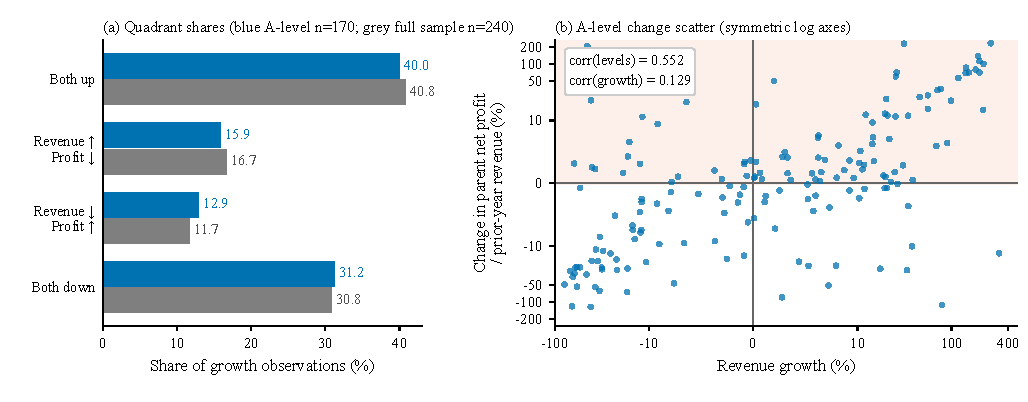
\includegraphics[width=0.95\textwidth]{../figures/en_fig2_quadrant.pdf}
\caption{Quadrants of revenue and profit changes, with A-level scatter. (a) Blue: 17 A-level firms ($n$ = 170 observations); grey: full sample ($n$ = 240). Quadrants are defined by the signs of the two level changes. (b) Scatter of revenue growth against the change in parent-attributable net profit scaled by prior-year revenue, on symmetric logarithmic axes; the sign of the vertical axis is that of the level change, so the upper-left region contains the divergent observations.}\label{fig:2}
\end{figure}

\subsection{Where the gap sits: two-period bridge}

Table 2 and Figure 3 present the period bridge. The common-firm sample contained 13 A-level firms observed in both subperiods, with n = 46 for 2015--2019 and n = 51 for 2020--2024. It is unbalanced at the firm-year level, so each period figure is a mean of the firm-years observed in that period rather than an equal-weighted mean of 13 firm means. Operating-layer margin increased from 30.60\% to 38.29\%, or 7.69 percentage points, while parent-attributable net margin fell from 11.19\% to \ensuremath{-}4.77\%, or \ensuremath{-}15.96 points.

\begin{table}[!htbp]
\centering
\caption{Two-period five-component decomposition of parent-attributable net margin (13 A-level firms observed in both subperiods; common-firm, unbalanced sample, \%).}\label{tab:2}
\begin{minipage}{\textwidth}
\centering
\footnotesize
\begin{adjustbox}{max width=\textwidth}
\begin{tabular}{@{}lrrr@{}}
\toprule
Component & 2015--2019 (n = 46) & 2020--2024 (n = 51) & Change \\
\midrule
Operating-layer margin & 30.60 & 38.29 & +7.69 \\
Minority interest & \ensuremath{-}1.48 & 1.50 & +2.98 \\
Interest burden & 4.80 & 6.86 & +2.06 \\
Impairment burden & 1.75 & 8.75 & +7.00 \\
Depreciation and amortisation intensity & 14.34 & 25.96 & +11.61 \\
\textbf{Parent-attributable net margin} & \textbf{11.19} & \textbf{\ensuremath{-}4.77} & \textbf{\ensuremath{-}15.96} \\
\bottomrule
\end{tabular}
\end{adjustbox}
\par\medskip
\raggedright
\noindent\textit{Notes.} The identity is: parent-attributable net margin = operating-layer margin \ensuremath{-} minority interest \ensuremath{-} interest burden \ensuremath{-} impairment burden \ensuremath{-} depreciation and amortisation intensity. It closes for every firm-year to a tolerance of 1e-9. The four deductions widened by 23.65 percentage points in total, which more than offset the 7.69-point improvement in the operating layer and produced a net decline of 15.96 points. The operating layer adds back interest, impairment and depreciation and amortisation but not income tax; it is therefore not EBITDA, and it is not statutory operating profit. The 13 firms are observed in both subperiods, but the panel is unbalanced at the firm-year level: 46 and 51 firm-years are pooled within each period, so the period figures are firm-year means and not equal-weighted means of 13 firm means.
\end{minipage}
\end{table}

Minority interest moved from \ensuremath{-}1.48\% to 1.50\% (+2.98 points), interest from 4.80\% to 6.86\% (+2.06), impairment from 1.75\% to 8.75\% (+7.00), and depreciation and amortisation from 14.34\% to 25.96\% (+11.61). The deductions increased by 23.65 points, closing the identity: 7.69 \ensuremath{-} 23.65 = \ensuremath{-}15.96. The operating layer improved while the parent-attributable margin fell; the gap was located below the operating layer, within these deductions. Their magnitudes identified accounting locations, not ranked causes.

\begin{figure}[!htbp]
\centering
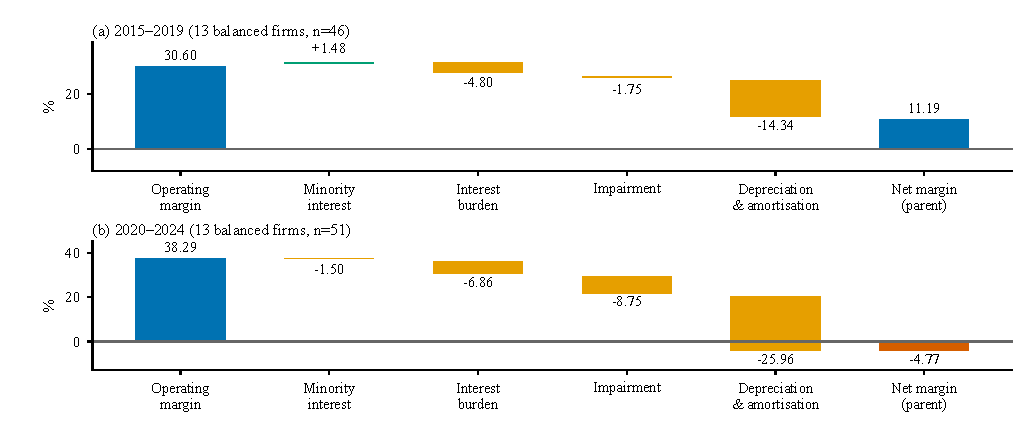
\includegraphics[width=0.95\textwidth]{../figures/en_fig3_waterfall.pdf}
\caption{Two-period waterfall of parent-attributable net margin (13 firms present in both subperiods). (a) 2015--2019 ($n$ = 46). (b) 2020--2024 ($n$ = 51). Minority interest of $-1.48$ appears as $+1.48$ because a subsidiary loss shared by minority shareholders is added back to the parent.}\label{fig:3}
\end{figure}

The unbalanced-sample check (Appendix Table A2), with n = 50/58, retained the directions but differed in magnitude because firm composition differed. Operating margin moved from 31.56\% to 34.91\% (+3.35 points), and net margin from 12.53\% to \ensuremath{-}3.67\% (\ensuremath{-}16.20). Minority interest changed from \ensuremath{-}1.09\% to 0.90\%, interest from 4.60\% to 6.18\%, impairment from 1.62\% to 7.74\%, and depreciation from 13.90\% to 23.76\%.

In the A-level frame retaining missing components, covering 156 firm-years, net margin fell from 11.58\% to \ensuremath{-}9.67\% (\ensuremath{-}21.25 points), while operating-layer margin moved from 27.39\% to 26.03\%. Zero substitution for missing components pulled deductions into the operating layer. This construction therefore could not confirm or reject the common-firm improvement; it illustrated how missing-data handling changed the accounting location assigned to the gap.

\subsection{Cross-section, loss years and the composition of deductions}

Figure 4 plots 2015--2024 firm means for the 17 A-level firms. Most points lie below the 45-degree line. Guilin Tourism recorded an operating layer of 52.22\% and a net margin of \ensuremath{-}29.39\%, a gap of 81.61 points accounted for by interest (12.97), impairment (19.85), depreciation (39.14) and minority interest (9.65). Zhangjiajie recorded an operating layer of 3.72\% and a net margin of \ensuremath{-}46.29\%, with depreciation of 36.12\%, the second highest among the 17 firms after Guilin Tourism. Qujiang Cultural Tourism recorded 13.43\% and \ensuremath{-}4.20\%. Emei Shan A recorded 38.04\% and 17.46\%, the exception in which a negative minority interest (\ensuremath{-}8.99\%) raised the parent margin. Similar gaps arose from different combinations of the four deductions, and the minority-interest sign was not uniform.

\begin{figure}[!htbp]
\centering
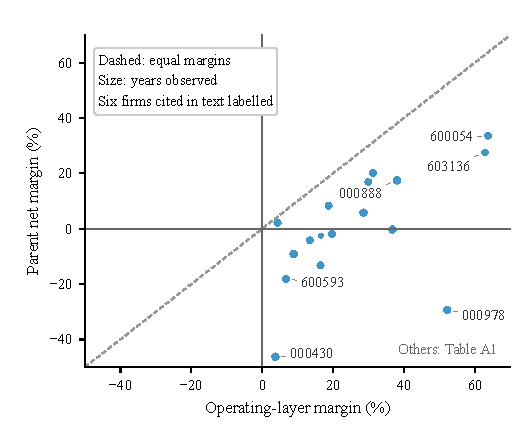
\includegraphics[width=0.80\textwidth]{../figures/en_fig4_firm_scatter.pdf}
\caption{Firm-level operating-layer margin and parent-attributable net margin (17 A-level firms; 2015--2024 means). The dashed line marks equality; point size indicates the number of observed years (5--10). Points below the line indicate that the deduction layer absorbed part of the operating return.}\label{fig:4}
\end{figure}

There were 67 loss firm-years, including 43 A-level observations. Across all loss years, mean net margin was \ensuremath{-}50.11\% and operating-layer margin was 11.98\%. Minority interest averaged 3.37\%, interest 10.26\%, impairment 27.20\%, depreciation 21.26\%, and gross deductions 58.73\%. For A-level loss years, mean net margin was \ensuremath{-}51.44\%, the operating layer \ensuremath{-}1.05\%, minority interest 2.39\%, interest 9.08\%, impairment 9.99\%, depreciation 28.93\% and gross deductions 48.01\%.

A negative operating layer occurred in 39.5\% of A-level loss years and 43.3\% of all loss years. The median loss-year net margin was \ensuremath{-}26.81\%, whereas the median operating layer was +3.68\%. Thus, a majority of loss observations retained a positive operating layer, with the accounting transition into loss occurring below that line. However, the A-level mean operating layer was slightly negative. The description of most loss years as operationally profitable applied to the median and observation share, not to the A-level mean.

Within gross deductions in loss years, impairment accounted for 46.3\%, depreciation for 36.2\%, and interest for 17.5\%. This composition described the distribution of deductions in loss observations, rather than their marginal associations with profitability.

\subsection{Why depreciation intensity rose: numerator or denominator?}

For the same 13-firm aggregation, depreciation intensity increased from 9.67\% to 19.34\%, a rise of 9.67 percentage points. Nominal depreciation increased by 43.2\%, contributing 4.18 points to the ratio change. Operating revenue declined by 28.4\%, contributing 3.83 points, while the interaction contributed 1.66 points.

This was an accounting decomposition of a ratio, not an attribution of cause. Both numerator growth and denominator contraction entered the arithmetic. The aggregate ratio of 9.67\% to 19.34\% differed in construction from the common-firm company-mean ratio of 14.34\% to 25.96\%. The former pooled amounts, whereas the latter described company-level margins; neither was used to corroborate the other.

\subsection{Contract design: fees, terms and sharing}

Table 3, Table 4 and Figure 5 present the contractual evidence. The corpus comprised 99 clauses from 7 firms and 32 reports, including 25 annual and 7 semi-annual reports covering 2016--2024. Merging repeated appearances yielded 39 agreement-level clauses. Of the original clauses, 94 appeared in the notes table headed `entrusted management/contracting', while 5 appeared under `other major contracts' in the main text.

\begin{table}[!htbp]
\centering
\caption{Disclosure channel by contract subject.}\label{tab:3}
\begin{minipage}{\textwidth}
\centering
\footnotesize
\begin{adjustbox}{max width=\textwidth}
\begin{tabular}{@{}lrrrr@{}}
\toprule
Subject & Notes table (all 94) & Of which annual records (78) & Main text, other major contracts (5) & Total (99) \\
\midrule
Other (asset, equity or management-rights custody) & 54 & 50 & 0 & 54 \\
Hotel & 26 & 18 & 0 & 26 \\
Travel agency & 13 & 9 & 0 & 13 \\
Scenic area & 0 & 0 & 5 & 5 \\
Port & 1 & 1 & 0 & 1 \\
Total & 94 & 78 & 5 & 99 \\
\bottomrule
\end{tabular}
\end{adjustbox}
\par\medskip
\raggedright
\noindent\textit{Notes.} One record corresponds to one agreement appearing in one report; an agreement repeated across years is counted once per report. The notes table refers to the standardised table on entrusted management/contracting and its counterpart; the main text refers to the section on major contracts and their performance, subsection 'other major contracts'. Subject is coded from the disclosed field rather than inferred from the firm name; the 32 records for 000524 describing 'management-rights custody' are therefore classified as 'other'.
\end{minipage}
\end{table}

Notes-table subjects comprised 54 `other' clauses covering asset, equity or management-rights custody, including 50 in annual reports; 26 hotel clauses, including 18 annual; 13 travel-agency clauses, including 9 annual; and 1 port clause. No scenic-area clause appeared in that channel. The main-text channel contained 5 scenic-area clauses, all from Qujiang.

\begin{table}[!htbp]
\centering
\caption{Five Qujiang agreements in the 2024 half-year report.}\label{tab:4}
\begin{minipage}{\textwidth}
\footnotesize
\begin{tabularx}{\textwidth}{@{}r >{\raggedright\arraybackslash}X >{\raggedright\arraybackslash}X r r r >{\raggedright\arraybackslash}p{2.0cm}@{}}
\toprule
No. & Principal & Subject & \shortstack{Fee recognised\\(RMB 10,000)} & \shortstack{Same-type\\share (\%)} & \shortstack{Revenue\\share (\%)} & Term \\
\midrule
1 & Xi'an Qujiang New District Social Undertaking Asset Management Centre & Tang Paradise & 2,541.41 & 5.23 & 3.30 & 2011-01-01\newline to 2030-12-31 \\
2 & Xi'an Qujiang New District Social Undertaking Asset Management Centre & Qujiang Pool and Tang City Wall Ruins Park & 2,359.51 & 4.86 & 3.06 & 2010-11-01\newline to 2030-10-31 \\
3 & Xi'an Qujiang New District Social Undertaking Asset Management Centre & Big Wild Goose Pagoda, Datang Never Night City (including Kaiyuan Square and Yintai Square) and Ci'en Temple Ruins Park & 511.27 & 1.05 & 0.66 & 2010-11-01\newline to 2030-10-31 \\
4 & Xi'an Qujiang Daminggong Ruins Area Protection and Reconstruction Office & Qujiang Daminggong Ruins Park & 6,798.50 & 14.00 & 8.83 & 2010-10-01\newline to 2030-09-30 \\
5 & Xi'an City Wall Development Management Co., Ltd. & Xi'an City Wall Scenic Area & 3,751.59 & 7.73 & 4.87 & 2018-10-01\newline to 2023-12-31 \\
\midrule
-- & Total & Five agreements & 15,962.28 & -- & 20.72 & -- \\
\bottomrule
\end{tabularx}
\par\medskip
\noindent\textit{Notes.} Amounts are recognised in the 2024 half-year and are not annualised. `Share of same-type transactions' reproduces the original disclosure; its denominator is same-type transaction value, not revenue. `Share of consolidated revenue' uses consolidated operating revenue of RMB 770,241,193.31 for the period. The five agreements total RMB 159.6228 million, or 20.72\% of half-year consolidated operating revenue. Agreement 5 is reported as disclosed: its stated term ended on 31 December 2023, yet RMB 3.7516 million was recognised under it in the 2024 half-year. The report discloses no renewal or extension, so the amount is retained as reported and the timing is flagged rather than explained.
\end{minipage}
\end{table}

For annual notes records (n = 78), the fee-to-revenue ratio had a median of 0.0101\%, a mean of 0.0343\% and a maximum of 0.8646\%. The largest single fee, RMB 16.8614 million, concerned entrusted operation of a port asset at 002627, not a scenic area. By contrast, Qujiang's five agreements totalled RMB 159.6228 million in the 2024 half-year against consolidated operating revenue of RMB 770,241,193.31, or 20.72\%. The same agreements totalled RMB 372.4894 million in the 2023 annual disclosure. The 2024 annual report marked the section `not applicable', so the half-year amount was not doubled or treated as comparable with annual totals.

\begin{figure}[!htbp]
\centering
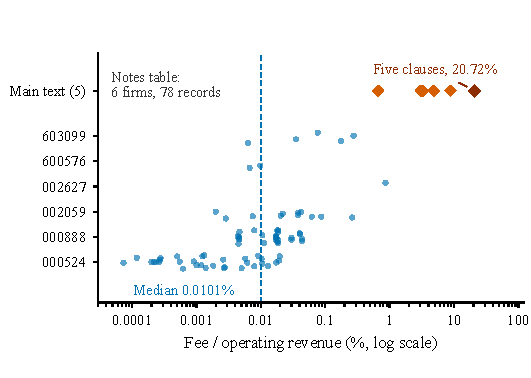
\includegraphics[width=0.80\textwidth]{../figures/en_fig5_fee_channel.pdf}
\caption{Fee-to-revenue ratios under two disclosure channels, on a logarithmic scale. The lower panel shows 78 annual notes-table records (median 0.0101\%); the upper panel shows the five Qujiang main-text clauses (20.72\% in aggregate).}\label{fig:5}
\end{figure}

Across these records, notes-table fees were tiny relative to the associated revenue, whereas the Qujiang main-text amount was approximately a fifth of consolidated revenue. This difference reflected disclosure channel and contractual subject, not competing estimates of the same quantity. The 20.72\% ratio was specific to Qujiang.

A determinable term was available for 53 of the 94 notes clauses. Of these, 48 were five years or less; the median was 2.92 years. Five exceeded five years, with a maximum of 10 years. The remaining 41 lacked an end date in the original disclosure. Only 7 of all 99 clauses contained a sharing formula.

Qujiang New District Social Undertaking Asset Management Centre used different regimes for different assets in the same city and period. For Qujiang Pool, Tang City Wall and Big Wild Goose Pagoda--Never Night City--Ci'en Temple, the operator's revenue entitlement followed a four-step schedule: 100\% in years 1--5, 92\% in years 6--10, 90\% in years 11--15 and 88\% in years 16--20. Contractual breakpoints fell in November 2020 and November 2025.

Tang Paradise had a basic fee of RMB 79.86 million, set on the 2019 ticket base and adjusted every three years. Excess-revenue bands specified no share at 0--10\%, 50/50 at 10--20\%, 60/40 at 20--30\%, 70/30 at 30--40\%, 80/20 at 40--50\%, and allocation entirely to the principal above 50\%. The operator's marginal share varied between 50\% and 80\% within the sharing bands and fell to zero beyond the top threshold.

Receivables exposed a separate settlement dimension. The Centre owed RMB 857,338,056.12, equivalent to 72.40\% of receivables plus contract assets, not revenue. Its bad-debt provision was RMB 257,201,416.84. The top five debtors totalled RMB 992,355,754.90 (83.80\%). A repayment plan dated 25 April 2025 scheduled RMB 924.90 million over five years, with RMB 228.50 million received as the first instalment.

Subsidiary results did not align monotonically with fee dependence. In the 2024 half-year, Daminggong reported revenue of RMB 67.985 million, fee/revenue of 100\% and net profit of \ensuremath{-}RMB 59.417 million. City Wall reported RMB 84.663 million, 44.31\% and +RMB 16.2725 million, respectively; Big Wild Goose Pagoda reported RMB 21.9656 million, 23.28\% and \ensuremath{-}RMB 7.6185 million. Datang Never Night City company reported revenue of RMB 39.383 million and net profit of +RMB 0.2353 million. Separately, the Never Night City block managed by the Big Wild Goose Pagoda subsidiary had a fee of RMB 5.1127 million. These distinct entity boundaries precluded conflation. Self-operated revenue was not sufficient for profitability, but the subsidiary contrast did not identify a causal effect.

\subsection{The disclosure-channel mismatch}

The absence of scenic-area subjects from all 94 notes clauses was not a sampling shortfall. Across 205 annual and semi-annual reports, only 6 firms and 31 reports, comprising 25 annual and 6 semi-annual reports, contained that notes table with data rows. All were read. Scenic-area agreements were visible in the main text but absent from the notes-table channel.

Coding also followed the disclosed field rather than an inferred business identity. The 32 records for 000524 described the subject only as `management-rights custody'; the entity name appeared in the principal column. Classification as `other' retained that distinction, rather than reconstructing the subject from the principal's name.

A notes-only contractual analysis would therefore have classified scenic-area concessions as absent from the sample despite their main-text disclosure. The channel mismatch constituted a measurement finding: the apparent contractual population depended on where the disclosure was read, not simply on the availability of reports.

\subsection{Cost obligations and net margins}

Table 5 and Figure 6 report the marginal associations. The main A-level specification included firm and year fixed effects, with standard errors clustered by firm across 17 clusters (n = 115, R\ensuremath{^2} = 0.646). Depreciation intensity carried a coefficient of +1.318, interest burden \ensuremath{-}3.772 and impairment \ensuremath{-}1.413. With 17 clusters the reference distribution matters. Under the conventional normal reference the p-values are 0.008, 0.047 and 0.029; under t with 16 degrees of freedom they are 0.017, 0.065 and 0.044; the CR2 variance estimator gives 0.018, 0.063 and 0.052; and a wild cluster bootstrap-t with 999 Rademacher draws and the null imposed gives 0.013, 0.063 and 0.011. We report the bootstrap p-values in the text and mark significance at the most conservative of the three references; Appendix Table A7 reports all four references and Appendix Table A8 the sample and window variants. Depreciation survives at the 5\% level; interest and impairment at the 10\% level.

\begin{table}[!htbp]
\centering
\caption{Three cost burdens and profitability (A-level firms, firm and year fixed effects, firm-clustered standard errors).}\label{tab:5}
\begin{minipage}{\textwidth}
\centering
\footnotesize
\textbf{Panel A.} Main specification.
\par\smallskip
\begin{tabular}{@{}lcc@{}}
\toprule
Independent variable & \shortstack{(1)\\Parent-attributable\\net margin} & \shortstack{(2)\\Operating cash-flow\\margin} \\
\midrule
Depreciation and amortisation/revenue & \shortstack{+1.318$^{**}$\\ (0.496)} & \shortstack{+1.947$^{***}$\\ (0.682)} \\
Interest burden & \shortstack{$-3.772^{*}$\\ (1.901)} & \shortstack{$-1.474$\\ (1.803)} \\
Impairment/revenue & \shortstack{$-1.413^{*}$\\ (0.647)} & \shortstack{$-0.967^{**}$\\ (0.395)} \\
$n$ & 115 & 115 \\
$R^{2}$ (within) & 0.646 & 0.591 \\
\bottomrule
\end{tabular}
\par\medskip
\textbf{Panel B.} Committed-stock specification (dependent variable: parent-attributable net margin).
\par\smallskip
\begin{tabular}{@{}lc@{}}
\toprule
Independent variable & \shortstack{Coefficient\\(standard error)} \\
\midrule
Interest-bearing debt/revenue & \shortstack{$-0.125^{*}$\\ (0.074)} \\
Long-term assets/revenue & \shortstack{+0.055\\ (0.039)} \\
Impairment/revenue & \shortstack{$-1.098$\\ (0.723)} \\
$n$ & 120 \\
$R^{2}$ (within) & 0.579 \\
\bottomrule
\end{tabular}
\par\medskip
\textbf{Panel C.} Turnover specification (dependent variable: parent-attributable net margin).
\par\smallskip
\begin{tabular}{@{}lc@{}}
\toprule
Independent variable & \shortstack{Coefficient\\(standard error)} \\
\midrule
Revenue/long-term assets & \shortstack{$-0.027$\\ (0.037)} \\
Interest burden & \shortstack{$-1.170$\\ (1.823)} \\
Impairment/revenue & \shortstack{$-1.371^{*}$\\ (0.781)} \\
$n$ & 115 \\
$R^{2}$ (within) & 0.573 \\
\bottomrule
\end{tabular}
\par\medskip
\raggedright
\noindent\textit{Notes.} Firm-clustered robust standard errors in parentheses, with the small-sample correction for 17 clusters. Because 17 clusters is few, three reference distributions are reported for column (1) in the text: the conventional normal, $t$ with 16 degrees of freedom, and a wild cluster bootstrap-$t$ with 999 Rademacher draws and the null imposed. Stars mark significance at the most conservative of the three: ** at the 5\% level and * at the 10\% level. In column (2) and in Panels B and C, stars follow the conventional normal reference and are descriptive only. A third column using the difference between parent-attributable net margin and operating cash-flow margin, reported in earlier drafts, is withdrawn: that difference is constructed from the same four deduction lines that enter the regressors, so its coefficients partly reproduce an accounting identity rather than an independent association. All variables are scaled by operating revenue and winsorised at $\pm$5\%. In Panel B, the long-term asset measure is not comparable before and after the new lease standard took effect in 2021; its coefficient is not interpreted economically.
\end{minipage}
\end{table}

For cash-flow margin (n = 115, R\ensuremath{^2} = 0.591), depreciation was +1.947 and impairment \ensuremath{-}0.967, both significant at the 5\% level or better under the conventional reference, whereas interest \ensuremath{-}1.474 was not descriptively significant. We do not report a specification with the net-margin-minus-cash-flow-margin difference as the dependent variable. That difference is constructed from the same four deduction lines that enter the regressors, so its coefficients partly reproduce an accounting identity rather than an independent association. An earlier draft reported one (n = 132) and we withdraw it for that reason.

\begin{figure}[!htbp]
\centering
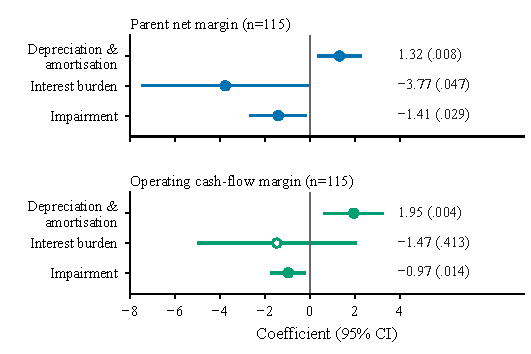
\includegraphics[width=0.80\textwidth]{../figures/en_fig6_forest.pdf}
\caption{Marginal associations of three cost burdens with profitability (A-level firms, controlling for firm and year effects). Each row corresponds to one regressor in a separate equation. Coefficients, intervals and the $p$-values printed at the right follow the conventional normal reference; filled markers denote $p<0.05$ under that reference. Because the panel has 17 clusters, inference in the text and in Table 5 uses the wild cluster bootstrap, under which interest burden is not significant at the 5\% level.}\label{fig:6}
\end{figure}

The stock specification (n = 120, R\ensuremath{^2} = 0.579) returned \ensuremath{-}0.125 for interest-bearing debt, +0.055 for long-term assets and \ensuremath{-}1.098 for impairment, none of which reaches the descriptive 5\% threshold; this specification did not add support. In the turnover specification (n = 115, R\ensuremath{^2} = 0.573), revenue/long-term assets was \ensuremath{-}0.027, interest \ensuremath{-}1.170 and impairment \ensuremath{-}1.371, the last significant at the 10\% level.

Sensitivity estimates retained the coefficient directions. In depreciation/interest/impairment order, baseline p-values were 0.008/0.047/0.029 (n = 115). Without year effects, coefficients were +1.012/\ensuremath{-}3.922/\ensuremath{-}1.668, with p = 0.146/0.066/0.008 (n = 115). Excluding 2022 yielded +1.908/\ensuremath{-}3.873/\ensuremath{-}1.435, with p < 0.001/p = 0.003/p = 0.029 (n = 103). Excluding 300144 and 000430 yielded +1.597/\ensuremath{-}4.068/\ensuremath{-}1.202, with p < 0.001/p = 0.037/p = 0.032 (n = 100). Depreciation weakened when year effects were removed. Three further checks bear on the 17-cluster problem. Restricting the window, depreciation was +1.452 (p = 0.008) over 2019--2024 and +0.442 (p = 0.314) over 2015--2018, while the interest coefficient changed sign; leaving out one firm at a time, depreciation kept its sign in all 17 re-estimations and stayed significant at the 5\% level in 16, impairment in 15 and interest in 3; adding capital expenditure intensity left all three coefficients in place (p = 0.051, 0.025 and 0.062). In the full sample (n = 176), only impairment remained descriptively significant, at \ensuremath{-}0.776 (p = 0.006); depreciation and interest were diluted. The A-level restriction was set before estimation on disclosure criteria --- continuous annual reports, a comparable statement template and identifiable deduction lines --- and not on the strength of the estimates. The full-sample result is reported alongside because it is substantively informative, and the weaker coefficients there are read as a loss of measurement precision rather than as evidence that the restricted sample is preferable.

One further check asks how much of the within-firm variation in profit growth the four deduction lines account for. On the 139 A-level observations with all four lines available, revenue growth alone explains almost none of that variation (R\ensuremath{^2} = 0.0013); adding the four burden changes raises R\ensuremath{^2} to 0.0390, so the increment is 0.0377 before and 0.0088 after adjustment for degrees of freedom, and a partial F test on the four added terms gives p = 0.272. Trimming the dependent variable at the 1st and 99th percentiles reverses the adjusted increment (\ensuremath{-}0.0189, p = 0.834). In the full sample (n = 201) the increment is 0.0167 before adjustment and \ensuremath{-}0.0031 after (p = 0.500). We read this as a bound on what the deduction lines can explain rather than as evidence for the mechanism. The burden variables are drawn from the same statements as the dependent variable, so they are not exogenous to it, and the increments are small against the variation they are meant to account for.

The positive depreciation coefficient may reflect a common-denominator effect rather than a profitability benefit from depreciation. The within-firm standard deviation of depreciation intensity was 1.33 times its between-firm standard deviation. In the aggregate decomposition of Section 4.4 the revenue decline contributed 3.83 of the 9.67-point rise, against 4.18 from nominal depreciation and 1.66 from their interaction, so the denominator accounts for about two-fifths of the movement rather than all of it. That decomposition describes an aggregate change, not the within-firm variation that identifies the coefficient. With year effects absorbing common shocks, remaining within-firm variation largely distinguished revenue above or below each firm's own mean. Depreciation intensity consequently behaved as an inverse proxy for capacity utilisation rather than a burden intensity. Removing year effects reduced the coefficient from +1.318 to +1.012 (p = 0.146), consistent with a substantial common-year component in the positive sign. This was a mechanical signature, not evidence that depreciation raised profitability.

Interest occupied the distribution stage: it was paid in cash but did not enter the operating section of the cash-flow statement. For a given operating cash flow, heavier interest corresponded to lower book profit through the accounting deduction. Its position was a value-capture leakage at distribution rather than an operating-cost squeeze. Impairment was a non-cash charge recognised below the constructed pre-deduction subtotal and was negatively associated with both book and cash margins; that association did not make it an operating cost. The coefficients occupied different income-statement positions, and their signs were read position by position.

\subsection{What the three layers do and do not establish}

The nominal-share layer described scale. Depreciation was the largest single deduction in 165 of 225 decomposition observations and represented 36\% of gross deductions. The period-change layer located the period gap: increases were ordered depreciation (+11.6 points), impairment (+7.0), minority interest (+3.0) and interest (+2.1). The marginal layer described within-firm co-movement: interest and impairment were negatively associated with net margin, whereas depreciation was positively associated.

These layers answered different questions and were reported side by side. The size of a deduction did not determine its period change or regression sign, and none of the layers was used to override another. Together, the evidence located the revenue--profit gap and its contractual correlates but did not identify exogenous causes. The small number of clusters (17) also meant that the reported p-values and asterisks were descriptive rather than a basis for strong inferential claims.

\section{Discussion and conclusion}

\subsection{From accounting leakage to asymmetric appropriation}

The contribution is not the discovery that costs matter, but the joint treatment of revenue rights and cost obligations. Value-capture accounts explain why actors may fail to appropriate value they help create, emphasising bargaining position, complementary assets and industry architecture (Bowman \& Ambrosini, 2000; Coff, 1999; Jacobides et al., 2006; Lepak et al., 2007). These accounts are usually applied to firms competing in markets. In the arrangements examined here, however, revenue entitlement is partly fixed through contracts with public principals, while the asset base and its financing remain with the listed operator. Increased activity can coexist with limited incremental appropriation. Where ownership is concentrated, the claims that sit in these deduction layers are also the classic channel through which controlling parties divert value (Johnson et al., 2000).

Property-rights reasoning clarifies why ownership of assets and entitlement to revenue streams can diverge (Grossman \& Hart, 1986; Hart, 1995). An operator may control day-to-day operations without holding a residual claim on incremental receipts. Revenue recognition then records activity without necessarily recording appropriation. The deterioration in parent-attributable net margins despite improvement at the operating layer is consistent with this distinction. It does not establish that contractual restrictions caused the deterioration, but indicates why operating performance alone is an incomplete measure of what shareholders retain.

``Revenue without residual claims'' is consequently a bounded construct, not a universal description of Chinese tourism. It applies where contractual schedules limit operators' shares of incremental revenue, asset-related obligations remain with operators, and public principals combine the roles of counterparty and pricing authority and, in some cases, debtor. The phrase captures an asymmetry between constrained revenue entitlement and continuing obligations, rather than suggesting that operators receive no income.

Read in this light, the evidence connects with public--private partnership research, which treats payment structures and risk allocation as interdependent design choices (Engel et al., 2014; Iossa \& Martimort, 2015). The evidence is consistent with that argument but does not test it causally. Nor should the construct be conflated with destination-level tourism leakage. That concept generally concerns value leaving a destination through imports, external ownership or repatriated profits. Here, accounting leakage concerns the passage from recognised revenue to retained profit within a listed operator's consolidated accounts, alongside contractual attenuation of its residual claim. The concepts concern different boundaries of appropriation and are related, not interchangeable.

\subsection{Three layers as a measurement protocol}

The three-layer approach separates questions that a single profitability indicator cannot answer. Nominal shares establish how large a deduction is relative to revenue. Period changes identify where the gap widened. Marginal associations indicate which burdens co-move with net margins within firms. Each perspective is informative, but each can mislead when treated as sufficient.

A nominal-share reading makes depreciation the dominant burden because it is the largest deduction. The period-change bridge also ranks depreciation first, followed by impairment, minority interest and interest. The panel instead associates interest and impairment negatively with net margins, while depreciation has a positive coefficient. These findings answer different questions rather than contradicting one another. In particular, the positive depreciation coefficient may reflect a common-denominator effect rather than a profitability benefit: revenue decline accounts for about two-fifths of the rise in depreciation intensity, and the coefficient falls when year effects are removed. Shared movements in revenue can alter the relationships between revenue-scaled variables without reversing the economic character of a cost.

The protocol is transferable to concessions, management contracts, franchising and platform intermediation, where recognised revenue and appropriation may similarly diverge. Its requirements are item-level financial statements and contract disclosure, rather than a particular national setting. Financial decomposition locates the deductions; contractual analysis helps establish who is entitled to receipts and responsible for obligations. Neither substitutes for the other.

Three cautions govern interpretation. The accounting identity closes by construction, so closure cannot validate the attribution of individual components. Substituting zero for missing components changes where the remaining gap is assigned, even when the identity balances. Finally, with only 17 firm clusters, panel p-values should be treated as descriptive rather than decisive evidence. The protocol organises evidence; it does not itself identify a contractual mechanism causally.

\subsection{Implications for operators, investors and public principals}

For operators, revenue and visitor growth are incomplete performance indicators when fees are fixed or marginal revenue shares decline. Reporting should place fee coverage, retained cost obligations and collection status alongside revenue. Such evidence would distinguish expanding activity from expanding capacity to finance maintenance and meet obligations. ``Asset-light'' descriptions require particular caution where depreciation, maintenance responsibilities and financing remain with the operator.

Investors should assess the contractual scope of the residual claim rather than assume that additional revenue accrues proportionately to shareholders. They should also read notes-table disclosures together with main-text major-contract sections. These channels yielded different contractual populations: scenic-area subjects were absent from the notes table but appeared in Qujiang's main-text disclosures. Reliance on either channel alone would therefore produce an incomplete exposure assessment. Receivables from public principals warrant separate attention because a recognised fee is not cash. The disclosed concentration of Qujiang's receivables makes collection status relevant independently of fee recognition or contractual entitlement.

For public principals, payment design determines whether additional activity generates a return for the operator that bears continuing obligations. Destination resources are frequently common-pool resources, and their governance depends on rules that allocate access, obligations and returns among users (Ostrom, 1990). A fee schedule is one such rule, and it can be evaluated as a governance instrument rather than only as a budget line. Transferring all incremental revenue above a threshold to the principal may increase its short-run share while weakening the operator's incentive to expand activity and its capacity to maintain assets. The evidence cannot quantify this trade-off, but identifies the relevant contractual margins: revenue-sharing thresholds, retained expenditure responsibilities and payment timing.

The disclosure-design implication is specific. In this sample, the notes-table template did not capture scenic-area concessions visible elsewhere in reports. Consistent subject categories across notes and main-text disclosures would make contractual exposure more visible to investors and regulators. This is a case for improving comparability and coverage, not a claim that existing disclosures are unlawful.

\subsection{Limitations and future research}

Causal identification is not supported by these findings. The panel is short, contractual exposure is not exogenous, and the contract sample is selected through disclosure. Firm and year fixed effects cannot remove all time-varying confounding or establish the counterfactual profitability of alternative contracts. The limited number of clusters further constrains inference.

Contract coverage is also narrow. The corpus contains 99 clauses from seven firms, but only seven records, covering four formula types, contain a sharing formula, and 41 lack a termination date. The absence of scenic-area subjects from the notes table indicates a disclosure-channel limitation, not the absence of such arrangements. The contractual evidence is illustrative and bounded, rather than representative of all Chinese scenic-area arrangements. It cannot establish the prevalence of the proposed configuration across the sector.

Measurement imposes additional qualifications. Ratios use operating revenue because reliable total-assets data are unavailable in the panel. This choice exposes estimates to denominator effects. The operating layer is measured after tax, with income tax not added back, and should not be interpreted as EBITDA. Missing components are set to zero and flagged. The accounting identity is not winsorised, whereas the regression is, so the decomposition and panel estimates serve different analytical purposes. The four deduction lines also account for little of the within-firm variation in profit growth: on the 139 A-level observations with complete deduction-line data, adding them to revenue growth moves R\ensuremath{^2} from 0.0013 to 0.0390 (the adjusted R\ensuremath{^2} changes by 0.0088, partial F p = 0.272), which bounds the mechanism as accounting-consistent rather than econometrically identified. Two further channels cannot be separated here. Reported profit remains open to real activities manipulation, so the deduction layer may reflect managerial choices alongside contractual obligations (Roychowdhury, 2006). Seasonal concentration of visits can also depress margins independently of contract terms (Cuccia \& Rizzo, 2011).

Destination-level value creation cannot be assessed with these data. Tourism activity also crosses administrative boundaries, so firm revenue records only the portion of destination demand that reaches the listed entity (Yang \& Fik, 2014). Without visitor spending, local procurement, employment or tax-revenue data, it observes only how much recognised revenue the listed operator retains. Weak shareholder appropriation need not imply weak destination benefits.

Future research should obtain contract-level fee schedules for a broader set of firms and estimate responses around contractual breakpoints. Linking visitor counts and destination spending to firm revenue would help separate demand expansion from capture. Comparisons between state-owned and privately owned operators could examine whether ownership conditions the configuration. Research could also test whether disclosure-channel differences affect investor pricing and extend the three-layer protocol to hotel management contracts, franchising and platform intermediation.

\subsection{Conclusion}

The paper begins with a persistent puzzle: recognised revenue can rise while net profit falls. Across the listed tourism firms examined, revenue and profit growth diverged, while the accounting bridge located the deterioration below an improving operating layer. Disclosed contracts are consistent with a configuration in which rights to incremental revenue and obligations associated with assets and financing are held asymmetrically by different parties.

``Revenue without residual claims'' summarises that configuration, subject to its contractual and institutional boundaries. It does not imply that contracts explain every profit decline, that all listed tourism firms face equivalent restrictions, or that tourism growth is illusory. Rather, it distinguishes expanding activity from the operator's ability to retain its proceeds.

The practical message is to assess revenue together with the contract governing it, the assets supporting it and the cash that actually arrives. This combined assessment offers a firmer basis for interpreting growth than revenue performance alone, without mistaking accounting reconciliation or disclosed contractual consistency for causal proof.

\FloatBarrier

\section*{CRediT authorship contribution statement}

\textbf{Yuan Zhao:} Conceptualization, Methodology, Formal analysis, Writing -- review \& editing, Project administration. \textbf{Yingtao Ji:} Data curation, Formal analysis, Investigation, Methodology, Writing -- original draft, Writing -- review \& editing, Funding acquisition. \textbf{Mengjie Hu:} Software, Methodology, Formal analysis, Investigation. \textbf{Songmei Liu:} Validation, Writing -- review \& editing, Supervision. \textbf{Chenyu Yang:} Data curation, Investigation, Validation.

\section*{Funding}

This research was supported by the Henan Federation of Social Sciences Research Project (2026, Grant No. SKL-2026-2533).

\section*{Declaration of competing interest}

The authors declare that they have no known competing financial interests or personal relationships that could have appeared to influence the work reported in this paper.

\section*{Data availability}

The firm-level panel is constructed from public annual and semi-annual reports. Derived variables, contract-coding records and estimation scripts are openly available in the replication repository at https://github.com/ristar2018/revenue-without-residual-claims, which maps every derived file to the script that produces it (Appendix Table A9). The source reports themselves remain subject to their publishers' terms of use. The contract corpus is limited to publicly disclosed clauses.


\section*{References}

\refitem{Abadie, A., Athey, S., Imbens, G. W., \& Wooldridge, J. M. (2023). When should you adjust standard errors for clustering? \emph{Quarterly Journal of Economics, 138}(1), 1--35. \url{https://doi.org/10.1093/qje/qjac038}}
\refitem{Airey, D., \& Chong, K. (2010). National policy-makers for tourism in China. \emph{Annals of Tourism Research, 37}(2), 295--314. \url{https://doi.org/10.1016/j.annals.2009.09.004}}
\refitem{Baker, G., Gibbons, R., \& Murphy, K. J. (2002). Relational contracts and the theory of the firm. \emph{The Quarterly Journal of Economics, 117}(1), 39--84. \url{https://doi.org/10.1162/003355302753399445}}
\refitem{Bianchi, R. (2018). The political economy of tourism development: A critical review. \emph{Annals of Tourism Research, 70}, 88--102. \url{https://doi.org/10.1016/j.annals.2017.08.005}}
\refitem{Blankespoor, E., Hendricks, B. E., Piotroski, J., \& Synn, C. (2022). Real-time revenue and firm disclosure. \emph{Review of Accounting Studies, 27}(3), 1079--1116. \url{https://doi.org/10.1007/s11142-022-09703-2}}
\refitem{Bowman, C., \& Ambrosini, V. (2000). Value creation versus value capture: Towards a coherent definition of value in strategy. \emph{British Journal of Management, 11}(1), 1--15. \url{https://doi.org/10.1111/1467-8551.00147}}
\refitem{Bramwell, B., \& Lane, B. (2011). Critical research on the governance of tourism and sustainability. \emph{Journal of Sustainable Tourism, 19}(4--5), 411--421. \url{https://doi.org/10.1080/09669582.2011.580586}}
\refitem{Cameron, A. C., Gelbach, J. B., \& Miller, D. L. (2008). Bootstrap-based improvements for inference with clustered errors. \emph{Review of Economics and Statistics, 90}(3), 414--427. \url{https://doi.org/10.1162/rest.90.3.414}}
\refitem{Cheong, C. S., Gao, S., Lun, P., Mihaylov, G., \& Zurbruegg, R. (2024). Biodiversity and the performance of tourism firms. \emph{Annals of Tourism Research, 109}, 103842. \url{https://doi.org/10.1016/j.annals.2024.103842}}
\refitem{Claessens, S., Djankov, S., \& Lang, L. H. P. (2000). The separation of ownership and control in East Asian corporations. \emph{Journal of Financial Economics, 58}(1--2), 81--112. \url{https://doi.org/10.1016/S0304-405X(00)00067-2}}
\refitem{Coff, R. W. (1999). When competitive advantage doesn't lead to performance: The resource-based view and stakeholder bargaining power. \emph{Organization Science, 10}(2), 119--133. \url{https://doi.org/10.1287/orsc.10.2.119}}
\refitem{Cuccia, T., \& Rizzo, I. (2011). Tourism seasonality in cultural destinations: Empirical evidence from Sicily. \emph{Tourism Management, 32}(3), 589--595. \url{https://doi.org/10.1016/j.tourman.2010.05.008}}
\refitem{Dechow, P., Ge, W., \& Schrand, C. (2010). Understanding earnings quality: A review of the proxies, their determinants and their consequences. \emph{Journal of Accounting and Economics, 50}(2--3), 344--401. \url{https://doi.org/10.1016/j.jacceco.2010.09.001}}
\refitem{Dewally, M., \& Gordon, R. (2022). Financial impact of partnerships on hospitality firms. \emph{Annals of Tourism Research, 95}, 103435. \url{https://doi.org/10.1016/j.annals.2022.103435}}
\refitem{Dwyer, L., Forsyth, P., \& Spurr, R. (2004). Evaluating tourism's economic effects: New and old approaches. \emph{Tourism Management, 25}(3), 307--317. \url{https://doi.org/10.1016/S0261-5177(03)00131-6}}
\refitem{Engel, E., Fischer, R., \& Galetovic, A. (2014). \emph{The economics of public--private partnerships: A basic guide}. Cambridge University Press. \url{https://doi.org/10.1017/CBO9781139565615}}
\refitem{Fan, J. P. H., Wong, T. J., \& Zhang, T. (2007). Politically connected CEOs, corporate governance, and post-IPO performance of China's newly partially privatized firms. \emph{Journal of Financial Economics, 84}(2), 330--357. \url{https://doi.org/10.1016/j.jfineco.2006.03.008}}
\refitem{Grossman, S. J., \& Hart, O. D. (1986). The costs and benefits of ownership: A theory of vertical and lateral integration. \emph{Journal of Political Economy, 94}(4), 691--719. \url{https://doi.org/10.1086/261404}}
\refitem{Hall, C. M. (2011). A typology of governance and its implications for tourism policy analysis. \emph{Journal of Sustainable Tourism, 19}(4--5), 437--457. \url{https://doi.org/10.1080/09669582.2011.570346}}
\refitem{Hart, O. (1995). \emph{Firms, contracts, and financial structure}. Oxford University Press. \url{https://doi.org/10.1093/0198288816.001.0001}}
\refitem{Hart, O. (2003). Incomplete contracts and public ownership: Remarks, and an application to public--private partnerships. \emph{The Economic Journal, 113}(486), C69--C76. \url{https://doi.org/10.1111/1468-0297.00119}}
\refitem{Hart, O., \& Moore, J. (1990). Property rights and the nature of the firm. \emph{Journal of Political Economy, 98}(6), 1119--1158. \url{https://doi.org/10.1086/261729}}
\refitem{He, Y., Wang, J., \& Meng, Q. (2025). The impact of mandatory operating information disclosure on related-party transactions: Evidence from China. \emph{Corporate Governance: An International Review, 33}(1), 103--124. \url{https://doi.org/10.1111/corg.12589}}
\refitem{Healy, P. M., \& Palepu, K. G. (2001). Information asymmetry, corporate disclosure, and the capital markets: A review of the empirical disclosure literature. \emph{Journal of Accounting and Economics, 31}(1--3), 405--440. \url{https://doi.org/10.1016/S0165-4101(01)00018-0}}
\refitem{International Accounting Standards Board. (2006). \emph{IFRIC 12: Service concession arrangements}. IFRS Foundation.}
\refitem{International Accounting Standards Board. (2014). \emph{IFRS 15: Revenue from contracts with customers}. IFRS Foundation.}
\refitem{International Accounting Standards Board. (2016). \emph{IFRS 16: Leases}. IFRS Foundation.}
\refitem{Iossa, E., \& Martimort, D. (2015). The simple microeconomics of public--private partnerships. \emph{Journal of Public Economic Theory, 17}(1), 4--48. \url{https://doi.org/10.1111/jpet.12114}}
\refitem{Jacobides, M. G., Knudsen, T., \& Augier, M. (2006). Benefiting from innovation: Value creation, value appropriation and the role of industry architectures. \emph{Research Policy, 35}(8), 1200--1221. \url{https://doi.org/10.1016/j.respol.2006.09.005}}
\refitem{Jensen, M. C., \& Meckling, W. H. (1976). Theory of the firm: Managerial behavior, agency costs and ownership structure. \emph{Journal of Financial Economics, 3}(4), 305--360. \url{https://doi.org/10.1016/0304-405X(76)90026-X}}
\refitem{Jiang, G., Lee, C. M. C., \& Yue, H. (2010). Tunneling through intercorporate loans: The China experience. \emph{Journal of Financial Economics, 98}(1), 1--20. \url{https://doi.org/10.1016/j.jfineco.2010.05.002}}
\refitem{Jin, H., Qian, Y., \& Weingast, B. R. (2005). Regional decentralization and fiscal incentives: Federalism, Chinese style. \emph{Journal of Public Economics, 89}(9--10), 1719--1742. \url{https://doi.org/10.1016/j.jpubeco.2004.11.008}}
\refitem{Jin, Y., Xi, H., Wang, X., Ren, X., \& Yuan, L. (2022). Evaluation of the integration policy in China: Does the integration of culture and tourism promote tourism development? \emph{Annals of Tourism Research, 97}, 103491. \url{https://doi.org/10.1016/j.annals.2022.103491}}
\refitem{Johnson, S., La Porta, R., Lopez-de-Silanes, F., \& Shleifer, A. (2000). Tunneling. \emph{American Economic Review, 90}(2), 22--27. \url{https://doi.org/10.1257/aer.90.2.22}}
\refitem{La Porta, R., Lopez-de-Silanes, F., \& Shleifer, A. (1999). Corporate ownership around the world. \emph{The Journal of Finance, 54}(2), 471--517. \url{https://doi.org/10.1111/0022-1082.00115}}
\refitem{Lepak, D. P., Smith, K. G., \& Taylor, M. S. (2007). Value creation and value capture: A multilevel perspective. \emph{Academy of Management Review, 32}(1), 180--194. \url{https://doi.org/10.5465/amr.2007.23464011}}
\refitem{Li, H., \& Zhou, L.-A. (2005). Political turnover and economic performance: The incentive role of personnel control in China. \emph{Journal of Public Economics, 89}(9--10), 1743--1762. \url{https://doi.org/10.1016/j.jpubeco.2004.06.009}}
\refitem{Li, H., He, L.-Y., \& Yang, J.-J. (2022). Forecasting the medium-term performance of restructured tourism firms with an adaptive integrated predictor. \emph{Tourism Management, 88}, 104436. \url{https://doi.org/10.1016/j.tourman.2021.104436}}
\refitem{Li, Y., \& Singal, M. (2019). Capital structure in the hospitality industry: The role of the asset-light and fee-oriented strategy. \emph{Tourism Management, 70}, 124--133. \url{https://doi.org/10.1016/j.tourman.2018.08.004}}
\refitem{Lim, S. E., \& Ok, C. M. (2021). A meta-analytic review of antecedents of hospitality and tourism firms' performance: A cross-cultural comparison. \emph{Tourism Management, 86}, 104325. \url{https://doi.org/10.1016/j.tourman.2021.104325}}
\refitem{Lussi, S., Masset, P., Weisskopf, J.-P., \& Blal, I. (2023). Cross-dimensional measures of asset lightness and fee orientation in lodging groups. \emph{International Journal of Hospitality Management, 109}, 103391. \url{https://doi.org/10.1016/j.ijhm.2022.103391}}
\refitem{Märklin, P., \& Bianchi, G. (2022). A differentiated approach to the asset-light model in the hotel industry. \emph{Cornell Hospitality Quarterly, 63}(3), 313--319. \url{https://doi.org/10.1177/19389655211006076}}
\refitem{Ministry of Finance of China. (2017). \emph{Accounting Standard for Business Enterprises No. 14: Revenue} (CAS 14). Ministry of Finance.}
\refitem{Ong, C.-E., \& Liu, Y. (2022). State-directed tourism urbanisation in China's Hengqin. \emph{Annals of Tourism Research, 94}, 103379. \url{https://doi.org/10.1016/j.annals.2022.103379}}
\refitem{Ostrom, E. (1990). \emph{Governing the commons: The evolution of institutions for collective action}. Cambridge University Press. \url{https://doi.org/10.1017/CBO9780511807763}}
\refitem{Peng, H., Zhang, J., Zhong, S., \& Li, P. (2021). Corporate governance, technical efficiency and financial performance: Evidence from Chinese listed tourism firms. \emph{Journal of Hospitality and Tourism Management, 48}, 163--173. \url{https://doi.org/10.1016/j.jhtm.2021.06.005}}
\refitem{Petersen, M. A. (2009). Estimating standard errors in finance panel data sets: Comparing approaches. \emph{Review of Financial Studies, 22}(1), 435--480. \url{https://doi.org/10.1093/rfs/hhn053}}
\refitem{Qian, Y., \& Weingast, B. R. (1997). Federalism as a commitment to preserving market incentives. \emph{Journal of Economic Perspectives, 11}(4), 83--92. \url{https://doi.org/10.1257/jep.11.4.83}}
\refitem{Roychowdhury, S. (2006). Earnings management through real activities manipulation. \emph{Journal of Accounting and Economics, 42}(3), 335--370. \url{https://doi.org/10.1016/j.jacceco.2006.01.002}}
\refitem{Schipper, K. (2007). Required disclosures in financial reports. \emph{The Accounting Review, 82}(2), 301--326. \url{https://doi.org/10.2308/accr.2007.82.2.301}}
\refitem{Shleifer, A., \& Vishny, R. W. (1997). A survey of corporate governance. \emph{The Journal of Finance, 52}(2), 737--783. \url{https://doi.org/10.1111/j.1540-6261.1997.tb04820.x}}
\refitem{Sigala, M. (2020). Tourism and COVID-19: Impacts and implications for advancing and resetting industry and research. \emph{Journal of Business Research, 117}, 312--321. \url{https://doi.org/10.1016/j.jbusres.2020.06.015}}
\refitem{Sohn, J., Tang, C.-H., \& Jang, S. (2013). Does the asset-light and fee-oriented strategy create value? \emph{International Journal of Hospitality Management, 32}, 270--277. \url{https://doi.org/10.1016/j.ijhm.2012.07.004}}
\refitem{Sun, K.-A., \& Lee, S. (2024). How do strategic pricing approaches influence franchise fee decisions? \emph{Tourism Economics, 30}(6), 1508--1530. \url{https://doi.org/10.1177/13548166231218766}}
\refitem{Teece, D. J. (1986). Profiting from technological innovation: Implications for integration, collaboration, licensing and public policy. \emph{Research Policy, 15}(6), 285--305. \url{https://doi.org/10.1016/0048-7333(86)90027-2}}
\refitem{Wang, D., \& Ap, J. (2013). Factors affecting tourism policy implementation: A conceptual framework and a case study in China. \emph{Tourism Management, 36}, 221--233. \url{https://doi.org/10.1016/j.tourman.2012.11.021}}
\refitem{Wang, T., Wu, P., Ge, Q., \& Ning, Z. (2021). Ticket prices and revenue levels of tourist attractions in China: Spatial differentiation between prefectural units. \emph{Tourism Management, 83}, 104214. \url{https://doi.org/10.1016/j.tourman.2020.104214}}
\refitem{Williamson, O. E. (1979). Transaction-cost economics: The governance of contractual relations. \emph{The Journal of Law and Economics, 22}(2), 233--261. \url{https://doi.org/10.1086/466942}}
\refitem{Williamson, O. E. (1985). \emph{The economic institutions of capitalism}. Free Press.}
\refitem{Yang, Y., \& Fik, T. (2014). Spatial effects in regional tourism growth. \emph{Annals of Tourism Research, 46}, 144--162. \url{https://doi.org/10.1016/j.annals.2014.03.007}}
\refitem{Yang, Y., Yao, C., \& Xu, D. (2020). Ecological compensation standards of national scenic spots in western China: A case study of Taibai Mountain. \emph{Tourism Management, 76}, 103950. \url{https://doi.org/10.1016/j.tourman.2019.103950}}

\clearpage
\section*{Appendix A. Supplementary table}

\begin{table}[!htbp]
\centering
\renewcommand{\thetable}{A1}
\caption{Sample firms, coverage and divergent firm-years.}\label{tab:A1}
\begin{minipage}{\textwidth}
\centering
\footnotesize
\begin{adjustbox}{max width=\textwidth}
\begin{tabular}{@{}lllrrrl@{}}
\toprule
Code & Firm & Tier & Firm-years & Calculable growth & Divergent & Principal segment \\
\midrule
000430 & Zhangjiajie Tourism Development & A & 11 & 10 & 2 & Zhangjiajie scenic area \\
000888 & Emei Shan Tourism & A & 11 & 10 & 0 & Mount Emei scenic area \\
000978 & Guilin Tourism & A & 11 & 10 & 1 & Guilin scenic area and cruise \\
002033 & Lijiang Yulong Tourism & A & 11 & 10 & 1 & Yulong Snow Mountain \\
002059 & Yunnan Tourism & A & 11 & 10 & 2 & Multiple sites, Yunnan \\
002159 & Sante Cableway & A & 11 & 10 & 3 & Cableways, multiple sites \\
002627 & Three Gorges Tourism & A & 11 & 10 & 1 & Ports and cruise, Hubei \\
300144 & Songcheng Performance & A & 11 & 10 & 1 & Theme parks, multiple sites \\
300859 & Western Regions Tourism & A & 11 & 10 & 1 & Tianchi, Xinjiang \\
600054 & Huangshan Tourism & A & 11 & 10 & 2 & Huangshan scenic area \\
600576 & Xiangyuan Culture and Tourism & A & 11 & 10 & 4 & Multiple sites \\
600593 & Dalian Sun Asia & A & 11 & 10 & 2 & Aquarium, Liaoning \\
600706 & Qujiang Cultural Tourism & A & 11 & 10 & 0 & Heritage parks, Xi'an \\
600749 & Tibet Tourism & A & 11 & 10 & 2 & Nyingchi, Tibet \\
603099 & Changbai Mountain Tourism & A & 11 & 10 & 4 & Changbai Mountain \\
603136 & Tianmu Lake Tourism & A & 11 & 10 & 1 & Tianmu Lake, Jiangsu \\
603199 & Jiuhua Mountain Tourism & A & 11 & 10 & 0 & Jiuhua Mountain, Anhui \\
000069 & OCT & B & 11 & 10 & 1 & Theme parks and property \\
000863 & Sanxiang Impression & B & 11 & 10 & 0 & Cultural shows and property \\
600138 & CYTS & B & 11 & 10 & 3 & Travel services and scenic sites \\
600358 & CITS Union & B & 11 & 10 & 3 & Travel services \\
000524 & Lingnan Holdings & C & 11 & 10 & 2 & Travel services, Guangdong \\
000721 & Xi'an Catering & C & 11 & 10 & 2 & Restaurants, Shaanxi \\
002707 & UTour Group & C & 11 & 10 & 2 & Outbound travel \\
\textbf{Total} & \textbf{24 firms} &  & \textbf{264} & \textbf{240} & \textbf{40} &  \\
\bottomrule
\end{tabular}
\end{adjustbox}
\par\medskip
\raggedright
\noindent\textit{Notes.} Firm-years cover 2015--2025. Calculable growth counts firm-years for which revenue and parent-attributable net profit are available in both the current and the preceding year. Divergent counts firm-years in which the level of revenue rose and the level of parent-attributable net profit fell. English names are working translations of the registered Chinese names and are used for identification only. Tier membership follows disclosure completeness and statement comparability, not financial performance.
\end{minipage}
\end{table}

\begin{table}[!htbp]
\centering
\renewcommand{\thetable}{A2}
\caption{Two-period five-component decomposition, unbalanced A-level sample (\%).}\label{tab:A2}
\begin{minipage}{\textwidth}
\centering
\footnotesize
\begin{adjustbox}{max width=\textwidth}
\begin{tabular}{@{}lrrr@{}}
\toprule
Component & 2015--2019 (n = 50) & 2020--2024 (n = 58) & Change \\
\midrule
Operating-layer margin & 31.56 & 34.91 & +3.35 \\
Minority interest & \ensuremath{-}1.09 & 0.90 & +1.99 \\
Interest burden & 4.60 & 6.18 & +1.58 \\
Impairment burden & 1.62 & 7.74 & +6.12 \\
Depreciation and amortisation intensity & 13.90 & 23.76 & +9.86 \\
\textbf{Parent-attributable net margin} & \textbf{12.53} & \textbf{\ensuremath{-}3.67} & \textbf{\ensuremath{-}16.20} \\
\bottomrule
\end{tabular}
\end{adjustbox}
\par\medskip
\raggedright
\noindent\textit{Notes.} Firms are not required to appear in both subperiods. The table tests whether the direction in Table 2 is an artefact of the 13-firm composition. The magnitude is slightly smaller (a net decline of 16.20 points), and the direction is unchanged.
\end{minipage}
\end{table}

\begin{table}[!htbp]
\centering
\renewcommand{\thetable}{A3}
\caption{Coding manual for contract clauses.}\label{tab:A3}
\begin{minipage}{\textwidth}
\centering
\footnotesize
\begin{adjustbox}{max width=\textwidth}
\begin{tabular}{@{}lll@{}}
\toprule
Column & Definition & Values or form \\
\midrule
code & Six-digit exchange code of the disclosing listed firm & 7 codes \\
year & Reporting year & 2016-2024 \\
kind & Report type & A (annual, 78 rows); H1 (semi-annual, 21 rows) \\
page & Page on which the entry appears in the layout text & integer \\
rec & Order of the entry within that page & 1-5 \\
channel & Location of the clause in the report & notes table (94); related-party main text (5) \\
counterparty & Principal that grants the revenue right & firm name, verbatim as disclosed \\
operator & Entity that receives the fee & firm name, verbatim; entries naming the disclosing firm itself are kept as disclosed \\
scope & Subject of the arrangement, standardised & operating-rights entrustment (33); hotel property (26); other asset entrustment (21); travel agency (13); equity entrustment (1); named scenic area (5) \\
scope\_raw & Subject as worded in the report & verbatim \\
start\_date & Start of the term as disclosed & YYYY-MM-DD \\
end\_date & End of the term as disclosed & YYYY-MM-DD; empty in 41 of 99 rows, meaning no end date is disclosed \\
pricing & Fee basis as worded in the report & verbatim excerpt \\
amount\_yuan & Fee recognised in the reporting period, RMB & numeric \\
nature & Sector of the subject & other (54); hotel (26); travel agency (13); scenic area (5); port (1) \\
pct\_same\_type & Share of same-type transactions, where the report states it & percent; stated for 5 of 99 rows \\
parse\_flag & Record of any cleaning applied during extraction & free text \\
note & Coder note & free text \\
\bottomrule
\end{tabular}
\end{adjustbox}
\par\medskip
\begin{adjustbox}{max width=\textwidth}
\begin{tabular}{@{}llll@{}}
\toprule
Code & Read from & Rule & Values \\
\midrule
Fee basis class & pricing & fixed sum; cost-based; revenue- or profit-sharing formula; stepwise or progressive schedule; not disclosed & 5 classes \\
Sharing & pricing & yes when the fee is a stated function of the counterparty's revenue or profit, no otherwise & yes; no \\
Termination disclosed & end\_date & yes when an end date is stated, no otherwise & yes; no \\
Agreement & counterparty + scope + start\_date & entries sharing all three are treated as one agreement & 39 agreements from 99 entries \\
\bottomrule
\end{tabular}
\end{adjustbox}
\par\medskip
\raggedright
\noindent\textit{Notes.} Chinese values are retained in the data files because they are the wording of the source notes; the replication package README lists their English equivalents, and the values printed in Panel A are those equivalents. Each clause was read in the original report. Ambiguities were resolved by re-reading the full contract description and the surrounding note rather than by interpreting an isolated table entry. Coding was carried out by a single coder, so no inter-coder reliability statistic is available; the manual is reported here so that the classification can be reproduced or challenged. A fee basis recorded as not disclosed means that the note states the existence of an arrangement without stating how the fee is calculated.
\end{minipage}
\end{table}

\begin{table}[!htbp]
\centering
\renewcommand{\thetable}{A4}
\caption{Search and screening yield for the contract sample.}\label{tab:A4}
\begin{minipage}{\textwidth}
\centering
\footnotesize
\begin{adjustbox}{max width=\textwidth}
\begin{tabular}{@{}lll@{}}
\toprule
Stage & Records & Basis \\
\midrule
Filings indexed & 43,906 & 24 firms, 1993--2026 \\
Reports retrieved & 311 & 226 annual and 85 semi-annual reports, 2015--2024 \\
Documents converted to layout text & 311 & page-level text with page marks retained \\
Page-level keyword hits & 1,180 & entrusted management, management fee, sharing, contracting out \\
Clause entries extracted & 99 & 94 notes-table entries and 5 related-party main-text entries \\
Firms and reports & 7 firms, 32 reports & disclosure units, not economic units \\
Agreement-level records & 39 & same counterparty, subject and start date \\
Entries with a fee-to-revenue ratio & 78 & annual entries with a fee and a firm-year revenue denominator \\
\bottomrule
\end{tabular}
\end{adjustbox}
\par\medskip
\raggedright
\noindent\textit{Notes.} The keyword search was run on the layout text of the 311 reports. A page-level hit is a page containing at least one search term; it is not a clause. Entries were retained only where the report states a fee amount or an explicit fee basis and identifies the counterparty and the subject. Related-party transactions that disclose a balance without a fee, and franchise arrangements that transfer a brand rather than a revenue right, were excluded. The yield from 1,180 page hits to 99 clause entries reflects this screening rather than a sampling design.
\end{minipage}
\end{table}

\begin{table}[!htbp]
\centering
\renewcommand{\thetable}{A5}
\caption{Clause inventory by firm.}\label{tab:A5}
\begin{minipage}{\textwidth}
\centering
\footnotesize
\begin{adjustbox}{max width=\textwidth}
\begin{tabular}{@{}llrrrllr@{}}
\toprule
Code & Firm & Records & Annual & Interim & Reporting years & Subjects & No end date \\
\midrule
000524 & Lingnan Holdings & 32 & 32 & 0 & 2017--2024 & Other asset (travel agencies) & 32 \\
000888 & Emei Shan Tourism & 39 & 27 & 12 & 2016--2024 & Hotel; travel agency & 0 \\
002059 & Yunnan Tourism & 14 & 11 & 3 & 2018--2022 & Other asset & 8 \\
002627 & Three Gorges Tourism & 1 & 1 & 0 & 2020 & Port & 1 \\
600576 & Xiangyuan Culture and Tourism & 3 & 2 & 1 & 2023--2024 & Hotel & 0 \\
600706 & Qujiang Cultural Tourism & 5 & 0 & 5 & 2024 & Scenic area & 0 \\
603099 & Changbai Mountain Tourism & 5 & 5 & 0 & 2024 & Other asset; equity & 0 \\
\textbf{Total} & \textbf{7 firms} & \textbf{99} & \textbf{78} & \textbf{21} & \textbf{2016--2024} &  & \textbf{41} \\
\bottomrule
\end{tabular}
\end{adjustbox}
\par\medskip
\raggedright
\noindent\textit{Notes.} Records are disclosure entries, so the same clause appears once for each report in which it is repeated. Seven records state a fee linked to revenue or profit by a formula, covering four formula types: 8\% of hotel revenue plus 5\% of operating profit (three records, one clause); a four-step entitlement of 100, 92, 90 and 88\% (two records, two parks under one agreement); a progressive excess schedule over a basic fee (one record); and retention of profit above a contracted target (one record). The remaining records state a fixed or cost-based amount, or refer to the notes without a formula. A missing end date is a property of the disclosure, not of the arrangement.
\end{minipage}
\end{table}

\begin{table}[!htbp]
\centering
\renewcommand{\thetable}{A6}
\caption{Typology of missing statement items.}\label{tab:A6}
\begin{minipage}{\textwidth}
\centering
\footnotesize
\begin{adjustbox}{max width=\textwidth}
\begin{tabular}{@{}lllr@{}}
\toprule
Class & Definition & Representative variables (missing firm-years) & Rows \\
\midrule
T1 & Institutional non-applicability: item introduced by an accounting standard after the observation year & right-of-use asset 83; lease liability 83; credit impairment 83 & 54 \\
T2 & Structural zero: item not applicable to the firm's business & bonds payable 186; goodwill 98; asset impairment 84 & 42 \\
T3 & Not separately presented: item exists but is not disclosed as a separate line & depreciation of fixed assets 130; cash paid to staff 118; intangible assets 80 & 90 \\
T4 & Collection gap: item is reported but was not captured & short-term loans 73; non-current liabilities due within one year 68; long-term loans 65 & 35 \\
T5 & Whole statement missing: 13 or more items absent in one firm-year & 4 firm-years (000069 in 2020; 002627 in 2017; 600358 in 2017 and 2018) & 4 \\
\textbf{Total} &  & \textbf{225 firm-years} & \textbf{225} \\
\bottomrule
\end{tabular}
\end{adjustbox}
\par\medskip
\raggedright
\noindent\textit{Notes.} A firm-year is assigned to the class that dominates its missing items. The T1 counts are firm-years before 2019, when the lease and financial-instrument standards took effect. Zero-fill sensitivity: setting all T1 and T2 items to zero returns 132 observations and leaves coefficient directions unchanged, with depreciation 0.758 (p = 0.150), interest \ensuremath{-}3.504 (p = 0.009) and impairment \ensuremath{-}1.049 (p = 0.008), against 1.318 (p = 0.008), \ensuremath{-}3.772 (p = 0.047) and \ensuremath{-}1.413 (p = 0.029) in the listwise sample of 115. Depreciation is therefore sensitive to the treatment of missing items and is reported as such.
\end{minipage}
\end{table}

\begin{table}[!htbp]
\centering
\renewcommand{\thetable}{A7}
\caption{Reference distributions for the cluster-robust estimates.}\label{tab:A7}
\begin{minipage}{\textwidth}
\centering
\footnotesize
\begin{adjustbox}{max width=\textwidth}
\begin{tabular}{@{}lrrrrrrr@{}}
\toprule
Regressor & Coefficient & Cluster SE & p (normal) & p t(G\ensuremath{-}1) & CR2 SE & p (CR2) & p (bootstrap) \\
\midrule
Depreciation intensity & 1.318 & 0.496 & 0.008 & 0.017 & 0.502 & 0.018 & 0.013 \\
Interest burden & \ensuremath{-}3.772 & 1.901 & 0.047 & 0.065 & 1.888 & 0.063 & 0.063 \\
Impairment burden & \ensuremath{-}1.413 & 0.647 & 0.029 & 0.044 & 0.672 & 0.052 & 0.011 \\
\bottomrule
\end{tabular}
\end{adjustbox}
\par\medskip
\raggedright
\noindent\textit{Notes.} n = 115, 17 clusters, R\ensuremath{^2} = 0.646. Each row is a separate equation with firm and year fixed effects. The bootstrap column reports a wild cluster bootstrap-t with 999 Rademacher draws and the null imposed. CR2 denotes the Imbens--Kolesár variance estimator. The three references disagree on interest burden at the 5\% level, which is why the text reports the bootstrap p-value and marks significance at the most conservative reference.
\end{minipage}
\end{table}

\begin{table}[!htbp]
\centering
\renewcommand{\thetable}{A8}
\caption{Sample and window variants of the three coefficients.}\label{tab:A8}
\begin{minipage}{\textwidth}
\centering
\footnotesize
\begin{adjustbox}{max width=\textwidth}
\begin{tabular}{@{}lrrrrrrr@{}}
\toprule
Regressor & Baseline & No year effects & Excluding 2022 & Excluding 300144 and 000430 & With capital expenditure & 2015--2018 & 2019--2024 \\
\midrule
Depreciation intensity & 1.318 (0.008) & 1.012 (0.146) & 1.908 (<0.001) & 1.597 (<0.001) & 1.084 (0.051) & 0.442 (0.314) & 1.452 (0.008) \\
Interest burden & \ensuremath{-}3.772 (0.047) & \ensuremath{-}3.922 (0.066) & \ensuremath{-}3.873 (0.003) & \ensuremath{-}4.068 (0.037) & \ensuremath{-}3.906 (0.025) & 1.883 (0.171) & \ensuremath{-}3.570 (0.134) \\
Impairment burden & \ensuremath{-}1.413 (0.029) & \ensuremath{-}1.668 (0.008) & \ensuremath{-}1.435 (0.029) & \ensuremath{-}1.202 (0.032) & \ensuremath{-}1.188 (0.062) & \ensuremath{-}0.382 (0.220) & \ensuremath{-}0.978 (0.182) \\
Observations & 115 & 115 & 103 & 100 & 115 & 44 & 71 \\
Clusters & 17 & 17 & 17 & 15 & 17 & 14 & 16 \\
\bottomrule
\end{tabular}
\end{adjustbox}
\par\medskip
\raggedright
\noindent\textit{Notes.} Coefficients with conventional cluster-robust p-values in parentheses. Leaving out one firm at a time, depreciation kept its sign in all 17 re-estimations and remained significant at the 5\% level in 16, impairment in 15 and interest in 3; the coefficient ranges were 1.023 to 1.686, \ensuremath{-}4.707 to \ensuremath{-}2.206 and \ensuremath{-}2.117 to \ensuremath{-}1.066. Capital expenditure intensity entered at 0.207 (p = 0.119). The period split is reported because the interest coefficient changes sign before 2019, which is consistent with the post-2019 rise in leverage in the panel rather than with a stable association across the whole window.
\end{minipage}
\end{table}

\begin{table}[!htbp]
\centering
\renewcommand{\thetable}{A9}
\caption{Reproduction map.}\label{tab:A9}
\begin{minipage}{\textwidth}
\centering
\footnotesize
\begin{adjustbox}{max width=\textwidth}
\begin{tabular}{@{}lll@{}}
\toprule
Artifact & File & Script \\
\midrule
Announcement index & data/ann\_index.csv & code/collect\_w1.py index \\
Annual and semi-annual reports & data/raw\_pdf/ & code/collect\_w1.py grab \\
Layout text & data/text/ & code/dump\_text.sh \\
Financial panel & data/panel\_annual\_2015\_2025\_v2.csv & vendor series, cross-checked \\
Statement-item panel & data/fin\_panel.csv & code/parse\_fin.py \\
Cross-check against the vendor series & data/fin\_vs\_em.csv & code/verify\_fin.py \\
Contract clauses & data/contract\_terms\_v4.csv & code/finalize\_contract4.py; code/add\_text\_contracts.py \\
Fee panel & data/contract\_fee\_panel.csv & code/contract\_summary.py \\
Cash-flow and depreciation panel & data/cashflow\_panel.csv & code/parse\_cashflow.py \\
Regression panel and estimates & data/h2\_panel.csv; data/h2\_results.csv & code/build\_h2.py \\
Robustness and inference references & data/h2\_robust.csv & code/h2\_robust.py \\
Incremental explanatory power & data/incremental\_r2.csv & code/incremental\_r2.py \\
Five-component decomposition & data/rq2\_decomp.csv & code/rq2\_decomp.py \\
Divergence counts & data/rq1\_stats.csv & code/rq1\_stats.py \\
Missing-data typology & data/miss\_typology.csv & code/miss\_typology.py \\
Figures & figures/ & code/figs.py; code/figs\_en.py; code/fig\_ga.py \\
Tables and manuscript & manuscript directory & code/assemble\_en.py; code/build\_tex\_en.py \\
\bottomrule
\end{tabular}
\end{adjustbox}
\par\medskip
\raggedright
\noindent\textit{Notes.} Scripts are Python 3.11 with pandas, numpy, scipy and statsmodels, except the layout-text conversion, which calls pdftotext. The wild cluster bootstrap uses Rademacher weights and a fixed seed, so the reported p-values are reproducible. Derived files are written to the paths listed; no step requires the raw PDFs once the layout text exists. The replication package accompanies the article and contains these files together with the coding manual of Table A3.
\end{minipage}
\end{table}

\end{document}
